\documentclass[11pt]{article}

% Change "review" to "final" for the camera-ready version.
% Change to "preprint" for a non-anonymous version with page numbers.
\usepackage[review]{acl}

\usepackage{times}
\usepackage{latexsym}
\usepackage[T1]{fontenc}
\usepackage[utf8]{inputenc}
\usepackage{microtype}
\usepackage{inconsolata}
\usepackage{amsmath}
\usepackage{booktabs}
\usepackage{graphicx}
\usepackage{rotating}
\usepackage{fancyvrb}
\usepackage{xspace}

\newcommand{\method}{FLIP\xspace}
\definecolor{promptborder}{RGB}{190,95,0}
\definecolor{promptfill}{RGB}{255,248,240}

\title{FLIP: A Flipped-Query Penalty for Negative-Constraint Retrieval}

\author{Anonymous Authors}

\begin{document}
\maketitle

\begin{abstract}
Users often express information needs with negative constraints.
Beyond explicit negation, queries may ask for answers that include one concept while excluding another, or for entities that belong to a category but differ from a closely related instance.
Because the excluded concept still appears in the query text, dense retrievers may assign high similarity to documents about that concept even when the user asks to avoid it.
We introduce \method, a training-free reranking method for negation-sensitive retrieval.
\method uses a large language model to extract a target query and a trap query for the excluded side, then penalizes documents similar to the trap query.
On ExcluIR, \method reduces trap retrieval across four embedding models with minimal loss in answer recall under selected penalty settings.
\end{abstract}

\section{Introduction}

Users often express information needs by specifying not only what should be retrieved, but also what should be avoided.
A query may ask for documents about one topic while excluding a related entity, or for items that belong to a category but differ from a particular instance.
For example, ``documentaries about the Iraq war, excluding \textit{Gunner Palace}'' asks the retriever to preserve the broad topic while avoiding a specific, highly related title.
When such documents are used as evidence in retrieval-augmented generation, an excluded document can enter the evidence context and cause the generator to ground its answer in material the user explicitly ruled out.

This setting is difficult for dense retrieval because the excluded concept is both salient and present in the query.
The retriever may assign high similarity to a document precisely because it matches the term the user asked to avoid, reflecting the lexical and semantic signals retained in dense representations \citep{ram-etal-2023-token}.
Negative queries with exclusion constraints therefore require a distinction between inclusion and exclusion semantics that standard retrievers often do not encode reliably \citep{lee2026deotrainingfreedirectembedding}.
Similar failures have also been observed in joint embedding-based vision-language retrieval, where models struggle to distinguish affirmative and negated conditions \citep{alhamoud2025visionlanguagemodelsunderstandnegation}.

Recent benchmarks and systems study this weakness across minimally different negated pairs, realistic negative queries with exclusion constraints, and negative-constraint retrieval \citep{weller-etal-2024-nevir, zhang2024excluir, xu-etal-2025-negconstraint}.
However, benchmarks with document-level answer and trap links remain scarce, and many existing approaches require specialized training data or model changes.
We study whether an existing retriever can be made more faithful to the exclusion constraint in a negative query at inference time, without retraining it.

We propose \method, a training-free reranking method for negative queries with exclusion constraints.
Given such a negative query, a large language model produces two short rewrites: a target query that preserves what should be retrieved and a trap query that names the forbidden intent.
\method then penalizes documents that are similar to the trap intent.
The language model is used only for query rewriting; it does not inspect documents, score candidates, or use gold answer and trap labels.

Our contributions are as follows.
\begin{itemize}
    \item We introduce \method, a training-free trap-penalty reranking method that changes only inference-time scores and requires no gold answer/trap labels, external knowledge, retriever retraining, or corpus modification.
    \item We formulate negative-constraint retrieval as a recall--violation trade-off and show that a trap-specific penalty can reduce excluded-document retrieval while preserving answer recall under suitable penalty strengths.
    \item We analyze when document-level trap penalties succeed or fail, identifying cases where relevant documents contain incidental trap evidence or lie close to trap documents in embedding space.
\end{itemize}

\section{Related Work}

\paragraph{Negative constraints in retrieval.}
Language models can be insensitive to negation and struggle to reason under negated statements \citep{truong-etal-2023-language}.
This weakness also appears in retrieval: NevIR tests minimally different negated pairs \citep{weller-etal-2024-nevir}, ExcluIR studies exclusion constraints with answer and trap documents \citep{zhang2024excluir}, BoolQuestions probes Boolean logic in dense retrieval \citep{zhang2024boolquestionsdoesdenseretrieval}, and NegConstraint applies neural-symbolic reranking for negative constraints \citep{xu-etal-2025-negconstraint}.
Similar support/contradiction confusion appears in biomedical QA when negation is central to the evidence \citep{sahoo2026negationsemanticdiagnosingdense}.

\paragraph{Embedding-level approaches to negation.}
A negated query still contains the entity or concept to be avoided, so dense encoders can place it near documents that violate the request.
DEO optimizes query embeddings at inference time for negation-aware retrieval \citep{lee2026deotrainingfreedirectembedding}; \method instead keeps retriever and document embeddings fixed and applies a score-level trap penalty.

\paragraph{Rank fusion for reranking.}
RRF combines ranked lists through reciprocal-rank contributions when raw scores are incomparable \citep{cormack2009reciprocal}.
We considered an anti-RRF variant that subtracts trap-query rank evidence, but use dense scores because they provide a smoother penalty signal.

\section{FLIP}

\method is a retrieval-time reranking method for negative queries with exclusion constraints.
It operates on fixed retriever scores by decomposing the query into target and trap intents, then lowering the rank of documents that are similar to the trap query.
In the main variant, \method uses the original query as the target-preserving signal and the decomposed trap intent as a penalty signal; a target-minus-trap variant is reported in the appendix.
The method consists of two steps: query decomposition and score transformation.

\begin{figure*}[t]
    \centering
    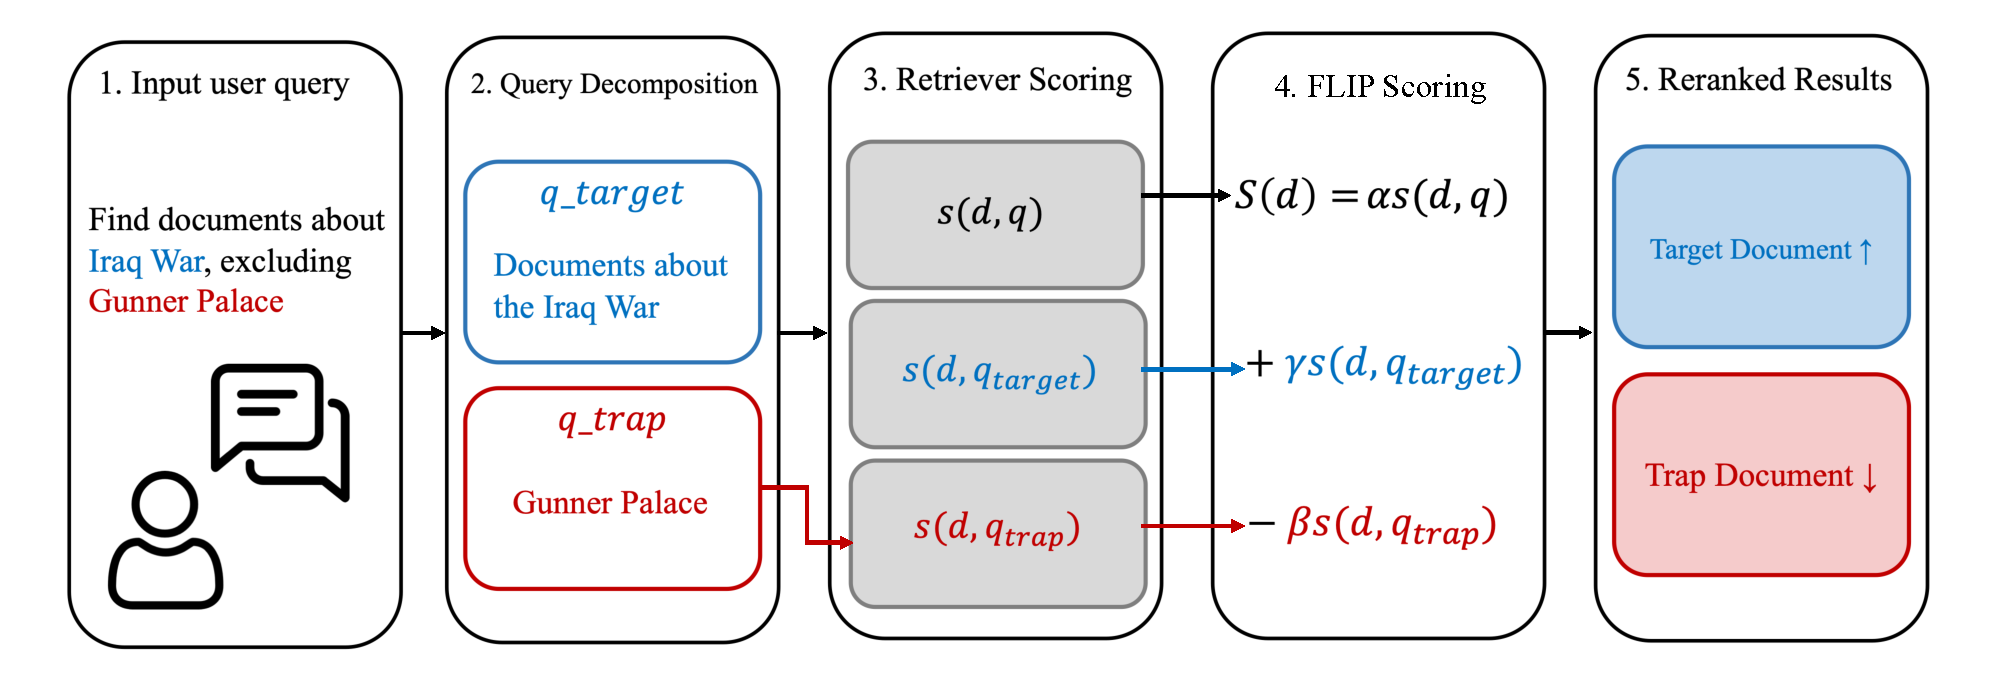
\includegraphics[width=0.96\textwidth]{figures/flip_pipeline_final_cropped.pdf}
    \caption{Overview of \method. A negative query with an exclusion constraint is decomposed into target and trap intents. The final document score preserves a positive retrieval signal while penalizing similarity to the trap intent.}
    \label{fig:flip-pipeline}
\end{figure*}

\subsection{Query Decomposition}

Let $q$ be a negative query that contains an exclusion constraint.
\method uses GPT-4o mini as the decomposer and asks it to produce two rewrites:
\begin{itemize}
    \item $q_{\mathrm{target}}$: the positive information need, with the exclusion removed but the main topic preserved;
    \item $q_{\mathrm{trap}}$: the forbidden intent that should be penalized.
\end{itemize}
Although many traps are named entities or titles, $q_{\mathrm{trap}}$ is not limited to entities: it may refer to an excluded concept, attribute, condition, or constraint.
For example, the query ``location of Friday Harbor Airport without bringing up Dayton International Airport'' is decomposed into target intent ``location of Friday Harbor Airport'' and trap intent ``Dayton International Airport''.
The LLM only produces these strings; it does not score documents, inspect the corpus, or use gold labels.
Appendix~\ref{sec:appendix-decomposition-prompt} provides the decomposition prompt.

\subsection{Score Transformation}

Let $s(d,q)$ be the retriever similarity score between document $d$ and query $q$.
The baseline ranks documents by $s(d,q)$, or by a cleaned rewrite of the original query when available.
\method uses dense similarity scores as a smoother penalty signal and computes
\begin{equation}
    S(d) = \alpha s(d,q) + \gamma s(d,q_{\mathrm{target}})
           - \beta s(d,q_{\mathrm{trap}}),
    \label{eq:flip}
\end{equation}
where $\alpha$, $\gamma$, and $\beta$ control the original-query, target, and trap terms.
We treat $(\alpha,\gamma)$ as a discrete choice rather than tuning them continuously: baseline-minus-trap uses $(1,0)$, and target-minus-trap uses $(0,1)$.
This isolates the effect of the trap penalty from changes caused by reweighting the positive retrieval signal.
The only tuned penalty weight is $\beta$, which controls how strongly documents similar to the trap query are demoted.
Table~\ref{tab:main-results} reports the baseline-minus-trap setting that preserves recall while reducing violation.
The appendix reports both scoring variants across beta values, with $\beta=0$ serving as the zero-penalty reference for each variant.
This formulation requires scores to be comparable across query rewrites; in this paper, we evaluate it with dense retriever scores.

\section{Experimental Setup}

\paragraph{Dataset.}
We evaluate on 3,452 negative queries with exclusion constraints from ExcluIR \citep{zhang2024excluir}.
Each example contains a rewritten exclusion query, a gold answer document, and a trap document corresponding to the excluded intent.
We score against the full ExcluIR corpus of 90,406 documents.
In our notation, the rewritten query is $q$, the answer-side document is $d_{\mathrm{target}}$, and the excluded-side document is $d_{\mathrm{trap}}$; $q_{\mathrm{target}}$ and $q_{\mathrm{trap}}$ are generated only from $q$ by the decomposer.
We use ExcluIR as the main benchmark because document-level target/trap annotations make recall and violation directly measurable, and report a smaller BoolQuestions-not auxiliary set in the appendix.
Appendix~\ref{sec:appendix-dataset-mapping} details the mapping from dataset fields to $q_{\mathrm{target}}$, $q_{\mathrm{trap}}$, $d_{\mathrm{target}}$, and $d_{\mathrm{trap}}$.

\paragraph{Retrievers and Decomposition.}
We test four embedding models: OpenAI text-embedding-3-small, OpenAI text-embedding-3-large, Qwen3-Embedding-0.6B, and Qwen3-Embedding-4B \citep{zhang2025qwen3embeddingadvancingtext}.
For each query, we generate $q_{\mathrm{target}}$ and $q_{\mathrm{trap}}$ with GPT-4o mini.
For the main variant, we use the original query as the positive retrieval signal and $q_{\mathrm{trap}}$ only as a penalty signal: $S(d)=s(d,q)-\beta s(d,q_{\mathrm{trap}})$.
We evaluate $\beta \in [0,1]$ at intervals of 0.01 to characterize the recall--violation trade-off rather than to claim a deployment-ready tuned hyperparameter.
Table~\ref{tab:main-results} reports the setting with the lowest average violation among settings that preserve average recall over $k \in \{3,5,7,9\}$ relative to the baseline.
Tables~\ref{tab:appendix-excluir-baseline-beta-000-049}--\ref{tab:appendix-excluir-target-beta-050-100} report the full ExcluIR results across penalty-weight settings, including the target-minus-trap variant.

\paragraph{Metrics.}
Recall@$k$ measures whether the gold answer document appears in the top $k$.
Violation@$k$ measures whether the trap document appears in the top $k$.
For retrieval with exclusion constraints, higher recall and lower violation are better.

\section{Results}

\begin{table*}[t]
\centering
\small
\begin{tabular}{llrrrrrr}
\toprule
Retriever & Method & $\beta$ & R@3 & V@3 & R@5 & V@5 & $\Delta$V@5 \\
\midrule
text-embedding-3-small & Baseline & -- & 0.9166 & 0.8250 & 0.9377 & 0.8789 & -- \\
text-embedding-3-small & \method & 0.32 & \textbf{0.9244} & \textbf{0.4287} & 0.9357 & \textbf{0.5165} & \textbf{-0.3624} \\
\midrule
text-embedding-3-large & Baseline & -- & 0.9270 & 0.8323 & 0.9400 & 0.8862 & -- \\
text-embedding-3-large & \method & 0.18 & \textbf{0.9273} & \textbf{0.6283} & 0.9397 & \textbf{0.7141} & \textbf{-0.1721} \\
\midrule
Qwen3-Embedding-0.6B & Baseline & -- & 0.9238 & 0.6654 & 0.9360 & 0.7277 & -- \\
Qwen3-Embedding-0.6B & \method & 0.06 & \textbf{0.9247} & \textbf{0.6011} & 0.9360 & \textbf{0.6611} & \textbf{-0.0666} \\
\midrule
Qwen3-Embedding-4B & Baseline & -- & 0.9282 & 0.6816 & 0.9421 & 0.7361 & -- \\
Qwen3-Embedding-4B & \method & 0.11 & \textbf{0.9296} & \textbf{0.5716} & \textbf{0.9424} & \textbf{0.6359} & \textbf{-0.1002} \\
\bottomrule
\end{tabular}
\caption{ExcluIR results on 3,452 queries over the full 90,406-document corpus. Only one representative $\beta$ setting is shown for each retriever: the setting with the lowest average violation among those preserving average recall relative to the baseline. R is recall, V is trap violation rate, and $\Delta$V@5 is \method{} V@5 minus baseline V@5 for the same retriever. Bold \method values improve on the corresponding baseline value.}
\label{tab:main-results}
\end{table*}

Table~\ref{tab:main-results} shows that \method reduces trap retrieval across all four retrievers.
The baselines achieve high recall but often retrieve the forbidden document as well, with violation@5 ranging from 0.728 to 0.886.
Increasing $\beta$ creates a clear recall--violation trade-off: stronger penalties demote trap documents, but very large penalties can also demote answer documents that share evidence with the trap intent.
At $\beta=1.0$, average violation drops to 0.030--0.036, but average recall falls to 0.779--0.835.

At the representative settings, average recall changes by at most 0.0002 from the baseline while average violation decreases for every retriever.
The largest top-$k$ reduction occurs for text-embedding-3-small, where violation@5 decreases from 0.879 to 0.517 while recall@5 changes only from 0.938 to 0.936.
The appendix shows the same beta-dependent trade-off across scoring variants, suggesting that the penalty strength should be selected for each retriever and scoring variant.

\section{Failure Analysis}

We manually inspected failure cases for the trap-penalty variant.
Two patterns dominate.
First, many gold answer documents mention the excluded entity.
For example, an answer page about a film may list an actor that the query asks to exclude.
Because \method applies a document-level penalty, such incidental trap evidence can lower otherwise correct documents.
Second, many answer and trap documents are close neighbors in embedding space: they often concern sibling entities, adaptations, cast members, or closely related institutions.
In these cases, the trap penalty can affect both documents.

These failures reflect the limits of a document-level penalty, not the reranking principle itself.
\method does not modify embeddings, but adjusts ranks at inference time by subtracting trap-specific similarity.
It works best when the trap signal is more specific to the excluded document than to the answer document.
When both documents share entities or lie close in embedding space, the penalty can affect both, suggesting the need for passage- or span-level evidence checks.

\section{Conclusion}

We presented \method, a training-free flipped-query penalty for negative queries with exclusion constraints.
By extracting a trap intent from the query and subtracting trap similarity, \method turns the exclusion constraint into a controllable score penalty.
Increasing $\beta$ strengthens the penalty on trap-like documents, which creates a recall--violation trade-off; however, our results show that suitable $\beta$ values can preserve answer recall while reducing trap retrieval.
This makes \method useful as an inference-time correction for existing dense retrievers, especially when retraining or changing the corpus is impractical.

\section*{Limitations}

\method is training-free because it does not update the retriever, require contrastive training, or construct additional supervision, but it incurs additional inference cost.
Inference adds query decomposition with an external language model, one extra retrieval or scoring pass for $q_{\mathrm{trap}}$, and linear reranking over candidates; the decomposition step can dominate latency and incur API cost.
We therefore frame \method as a reranking method with no training cost, leaving latency--cost evaluation and compact local decomposition models to future work.
\method also assumes that decompositions are reliable and that retriever scores are comparable across target and trap queries.
The reported settings characterize the trade-off on the evaluated sample rather than a deployment-tuned operating point; in practice, $\beta$ should be selected on a held-out validation split.
Our main evaluation is limited to ExcluIR and dense retrieval because few benchmarks provide both target and trap documents; rather than generating synthetic trap documents with an LLM, we use existing annotations so violation measurement remains grounded in benchmark evidence.
Additional evaluations should include sparse retrieval, cross-encoder reranking, and downstream RAG answer quality.
Because \method applies a document-level penalty, it can be less precise when relevant documents incidentally mention the excluded entity or closely overlap with trap documents.
Future work can combine \method with passage- or span-level checks to separate central trap evidence from incidental mentions.

\clearpage
\bibliography{custom}

\clearpage
\appendix

\section{Experimental Details}

\paragraph{Compute.}
All experiments were run on a single RTX 4090 GPU with 16 vCPUs (AMD Ryzen 9 7950X 16-Core Processor), 61 GB memory, and a 20 GB container disk.

\section{Query Decomposition Prompt}
\label{sec:appendix-decomposition-prompt}

The template below was used with GPT-4o mini at temperature 0 to generate
$q_{\mathrm{target}}$ and $q_{\mathrm{trap}}$.

\begin{figure*}[p]
\centering
\begingroup
\setlength{\fboxsep}{0pt}
\fcolorbox{promptborder}{promptfill}{%
\begin{minipage}{0.96\linewidth}
\colorbox{promptborder}{%
\begin{minipage}{\dimexpr\linewidth-2\fboxsep\relax}
\textcolor{white}{\textbf{Query Decomposition Prompt Template}}
\end{minipage}}
\vspace{0.6em}
\begin{minipage}{0.94\linewidth}
\small
\textbf{Role:}
You are a recall-preserving query decomposition module for
exclusion-aware information retrieval.

\textbf{Task:}
Given only the original query, produce two retrieval queries:
$q_{\mathrm{target}}$, the positive information need, and
$q_{\mathrm{trap}}$, a short high-precision anchor for the unwanted,
excluded, contrastive, or constraint-violating side.
Do not use gold documents, trap documents, answers, relevance labels,
dataset annotations, or external knowledge beyond what is directly implied
by the query.

\textbf{Decomposition Rules:}
Preserve the main search intent in $q_{\mathrm{target}}$ and remove only
phrases that point to the unwanted side.
$q_{\mathrm{target}}$ should remain independently useful for retrieval and
should not encode the exclusion with wrappers such as ``not'', ``without'',
``excluding'', ``except'', ``instead of'', or ``rather than'', unless the
negated phrase is the natural name of the desired concept.
$q_{\mathrm{trap}}$ should be the strongest compact retrieval anchor for
the unwanted side: preferably an explicitly excluded named entity, title,
organization, person, work, place, product, event, date, object, attribute,
condition, relation, role, or category.
Strip exclusion wrappers from $q_{\mathrm{trap}}$ and avoid broad anchors
such as ``career'', ``film'', ``country'', or ``person'' unless the unwanted
side is exactly that broad.
If the query contains a direct contrast, use the obvious counterpart when
available (e.g., legal $\leftrightarrow$ illegal, allowed
$\leftrightarrow$ forbidden, paid $\leftrightarrow$ unpaid, present
$\leftrightarrow$ absent, won $\leftrightarrow$ lost).
If no direct counterpart is obvious, use the explicit unwanted phrase.
Set $q_{\mathrm{trap}}$ to an empty string only when no excluded,
negative, contrastive, exception, or undesired side is present.

\textbf{Output Format:}
Return only valid JSON with exactly two fields:

\noindent{\ttfamily\scriptsize
\{\\
\hspace*{1em}"q\_target": "...",\\
\hspace*{1em}"q\_trap": "..."\\
\}
}

\textbf{User Message Template:}

\noindent{\ttfamily\scriptsize
Now decompose the following query.\\[0.2em]
Original query:\\
\{original\_query\}\\[0.2em]
Return only valid JSON. Do not include markdown, comments,
explanations, or extra fields.\\[0.2em]
\{\\
\hspace*{1em}"q\_target": "...",\\
\hspace*{1em}"q\_trap": "..."\\
\}
}
\end{minipage}
\vspace{0.7em}
\end{minipage}}
\endgroup
\end{figure*}

\clearpage
\section{Dataset Mapping and Auxiliary Set}
\label{sec:appendix-dataset-mapping}

ExcluIR provides a natural four-part structure for our setting.
The rewritten exclusion query is $q$, the answer-side corpus index is $d_{\mathrm{target}}$, and the excluded-side corpus index is $d_{\mathrm{trap}}$.
Its paired construction also makes oracle-style query anchors recoverable: the original positive question can be viewed as $q_{\mathrm{target}}$, and the title or short identifier of the excluded document can be viewed as $q_{\mathrm{trap}}$.
In the reported \method experiments, however, $q_{\mathrm{target}}$ and $q_{\mathrm{trap}}$ are generated only from $q$ by GPT-4o mini; gold document indices are used only for evaluation.

For other negative-constraint retrieval datasets, $q_{\mathrm{target}}$ is the positive information need after removing the exclusion, $q_{\mathrm{trap}}$ is the compact forbidden anchor, $d_{\mathrm{target}}$ is a document satisfying the positive need, and $d_{\mathrm{trap}}$ is a plausible but constraint-violating document.
When a dataset provides positive and negative passages, we map them to $d_{\mathrm{target}}$ and $d_{\mathrm{trap}}$ respectively.
When it provides only documents, $q_{\mathrm{target}}$ and $q_{\mathrm{trap}}$ can be produced by the same query-only decomposer.

As an auxiliary check, we evaluate the subset of BoolQuestions \citep{zhang2024boolquestionsdoesdenseretrieval} with \texttt{question\_type = not}.
Each example includes a positive passage and a negative passage that can be treated as $d_{\mathrm{target}}$ and $d_{\mathrm{trap}}$.
This yields 323 examples, 195 from MS MARCO and 128 from Natural Questions, over a 646-document evaluation corpus.
Because BoolQuestions does not provide explicit $q_{\mathrm{target}}$ and $q_{\mathrm{trap}}$ fields, we generate them with the same GPT-4o mini decomposer and report results across penalty-weight settings in Tables~\ref{tab:appendix-boolquestions-baseline-beta-000-049}--\ref{tab:appendix-boolquestions-target-beta-050-100}.

% Auto-generated from paper beta results. Do not edit by hand.
\section{Additional Results}
\noindent Tables~\ref{tab:appendix-excluir-baseline-beta-000-049}--\ref{tab:appendix-boolquestions-target-beta-050-100} report the full beta grid for the baseline-minus-trap and target-minus-trap scoring variants.

\begin{sidewaystable*}[p]
\centering
\begingroup
\scriptsize
\setlength{\tabcolsep}{1.70pt}
\renewcommand{\arraystretch}{0.74}
\begin{tabular}{@{}r*{16}{r}@{}}
\toprule
$\beta$ & \multicolumn{4}{c}{te3-small} & \multicolumn{4}{c}{te3-large} & \multicolumn{4}{c}{Qwen3-Embedding-0.6B} & \multicolumn{4}{c}{Qwen3-Embedding-4B} \\
\cmidrule(lr){2-5} \cmidrule(lr){6-9} \cmidrule(lr){10-13} \cmidrule(lr){14-17}
 & R@5 & V@5 & Avg. R & Avg. V & R@5 & V@5 & Avg. R & Avg. V & R@5 & V@5 & Avg. R & Avg. V & R@5 & V@5 & Avg. R & Avg. V \\
\midrule
0.00 & 0.9377 & 0.8789 & 0.9366 & 0.8788 & 0.9400 & 0.8862 & 0.9412 & 0.8871 & 0.9360 & 0.7277 & 0.9383 & 0.7320 & 0.9421 & 0.7361 & 0.9422 & 0.7412 \\
0.01 & 0.9383 & 0.8737 & 0.9366 & 0.8730 & 0.9400 & 0.8786 & 0.9413 & 0.8800 & 0.9354 & 0.7178 & 0.9382 & 0.7223 & 0.9418 & 0.7294 & 0.9423 & 0.7338 \\
0.02 & 0.9386 & 0.8627 & 0.9368 & 0.8658 & 0.9406 & 0.8714 & 0.9416 & 0.8737 & 0.9360 & 0.7060 & 0.9382 & 0.7134 & 0.9418 & 0.7239 & 0.9424 & 0.7269 \\
0.03 & 0.9383 & 0.8557 & 0.9371 & 0.8583 & 0.9415 & 0.8653 & 0.9417 & 0.8667 & 0.9351 & 0.6961 & 0.9382 & 0.7034 & 0.9418 & 0.7149 & 0.9425 & 0.7184 \\
0.04 & 0.9380 & 0.8488 & 0.9371 & 0.8517 & 0.9421 & 0.8586 & 0.9418 & 0.8594 & 0.9351 & 0.6845 & 0.9382 & 0.6932 & 0.9418 & 0.7028 & 0.9426 & 0.7094 \\
0.05 & 0.9377 & 0.8407 & 0.9374 & 0.8452 & 0.9421 & 0.8525 & 0.9419 & 0.8532 & 0.9354 & 0.6715 & 0.9380 & 0.6811 & 0.9415 & 0.6955 & 0.9424 & 0.7010 \\
0.06 & 0.9371 & 0.8340 & 0.9370 & 0.8380 & 0.9421 & 0.8465 & 0.9421 & 0.8461 & 0.9360 & 0.6611 & 0.9383 & 0.6701 & 0.9412 & 0.6840 & 0.9423 & 0.6895 \\
0.07 & 0.9371 & 0.8256 & 0.9372 & 0.8280 & 0.9421 & 0.8395 & 0.9421 & 0.8401 & 0.9360 & 0.6527 & 0.9380 & 0.6601 & 0.9412 & 0.6747 & 0.9421 & 0.6779 \\
0.08 & 0.9374 & 0.8149 & 0.9376 & 0.8191 & 0.9424 & 0.8320 & 0.9422 & 0.8326 & 0.9354 & 0.6451 & 0.9377 & 0.6490 & 0.9418 & 0.6637 & 0.9420 & 0.6685 \\
0.09 & 0.9377 & 0.8056 & 0.9379 & 0.8095 & 0.9421 & 0.8227 & 0.9421 & 0.8233 & 0.9354 & 0.6341 & 0.9376 & 0.6384 & 0.9421 & 0.6547 & 0.9422 & 0.6587 \\
0.10 & 0.9377 & 0.7961 & 0.9379 & 0.8001 & 0.9415 & 0.8108 & 0.9424 & 0.8132 & 0.9354 & 0.6202 & 0.9374 & 0.6262 & 0.9421 & 0.6446 & 0.9424 & 0.6485 \\
0.11 & 0.9377 & 0.7839 & 0.9382 & 0.7896 & 0.9412 & 0.7966 & 0.9423 & 0.8016 & 0.9345 & 0.6086 & 0.9371 & 0.6154 & 0.9424 & 0.6359 & 0.9423 & 0.6388 \\
0.12 & 0.9380 & 0.7726 & 0.9385 & 0.7791 & 0.9412 & 0.7859 & 0.9424 & 0.7898 & 0.9345 & 0.5976 & 0.9367 & 0.6034 & 0.9421 & 0.6266 & 0.9420 & 0.6284 \\
0.13 & 0.9386 & 0.7613 & 0.9387 & 0.7696 & 0.9415 & 0.7738 & 0.9426 & 0.7793 & 0.9342 & 0.5869 & 0.9364 & 0.5944 & 0.9415 & 0.6159 & 0.9416 & 0.6198 \\
0.14 & 0.9389 & 0.7457 & 0.9387 & 0.7565 & 0.9415 & 0.7633 & 0.9422 & 0.7682 & 0.9342 & 0.5771 & 0.9361 & 0.5839 & 0.9412 & 0.6040 & 0.9416 & 0.6094 \\
0.15 & 0.9383 & 0.7346 & 0.9386 & 0.7444 & 0.9409 & 0.7483 & 0.9421 & 0.7551 & 0.9340 & 0.5660 & 0.9357 & 0.5716 & 0.9406 & 0.5933 & 0.9413 & 0.5994 \\
0.16 & 0.9377 & 0.7248 & 0.9383 & 0.7318 & 0.9403 & 0.7396 & 0.9420 & 0.7435 & 0.9340 & 0.5542 & 0.9357 & 0.5590 & 0.9406 & 0.5823 & 0.9410 & 0.5886 \\
0.17 & 0.9371 & 0.7126 & 0.9379 & 0.7194 & 0.9403 & 0.7268 & 0.9416 & 0.7311 & 0.9337 & 0.5435 & 0.9356 & 0.5476 & 0.9406 & 0.5730 & 0.9408 & 0.5775 \\
0.18 & 0.9374 & 0.7002 & 0.9379 & 0.7082 & 0.9397 & 0.7141 & 0.9414 & 0.7191 & 0.9337 & 0.5310 & 0.9351 & 0.5376 & 0.9403 & 0.5614 & 0.9407 & 0.5674 \\
0.19 & 0.9377 & 0.6880 & 0.9379 & 0.6955 & 0.9392 & 0.7019 & 0.9409 & 0.7071 & 0.9337 & 0.5180 & 0.9350 & 0.5261 & 0.9397 & 0.5527 & 0.9403 & 0.5573 \\
0.20 & 0.9377 & 0.6753 & 0.9375 & 0.6842 & 0.9392 & 0.6889 & 0.9408 & 0.6943 & 0.9334 & 0.5061 & 0.9345 & 0.5147 & 0.9403 & 0.5411 & 0.9402 & 0.5456 \\
0.21 & 0.9380 & 0.6608 & 0.9375 & 0.6704 & 0.9389 & 0.6773 & 0.9407 & 0.6818 & 0.9331 & 0.4933 & 0.9342 & 0.5030 & 0.9403 & 0.5293 & 0.9403 & 0.5347 \\
0.22 & 0.9380 & 0.6521 & 0.9375 & 0.6580 & 0.9397 & 0.6648 & 0.9409 & 0.6685 & 0.9325 & 0.4852 & 0.9338 & 0.4915 & 0.9395 & 0.5159 & 0.9401 & 0.5237 \\
0.23 & 0.9377 & 0.6402 & 0.9375 & 0.6454 & 0.9403 & 0.6503 & 0.9410 & 0.6544 & 0.9325 & 0.4731 & 0.9337 & 0.4803 & 0.9392 & 0.5038 & 0.9397 & 0.5125 \\
0.24 & 0.9374 & 0.6301 & 0.9375 & 0.6334 & 0.9406 & 0.6362 & 0.9409 & 0.6401 & 0.9325 & 0.4618 & 0.9332 & 0.4686 & 0.9395 & 0.4974 & 0.9397 & 0.5026 \\
0.25 & 0.9371 & 0.6173 & 0.9371 & 0.6204 & 0.9415 & 0.6214 & 0.9408 & 0.6252 & 0.9322 & 0.4528 & 0.9329 & 0.4570 & 0.9395 & 0.4884 & 0.9398 & 0.4923 \\
0.26 & 0.9366 & 0.5982 & 0.9366 & 0.6057 & 0.9412 & 0.6063 & 0.9406 & 0.6114 & 0.9319 & 0.4415 & 0.9326 & 0.4463 & 0.9389 & 0.4806 & 0.9399 & 0.4833 \\
0.27 & 0.9368 & 0.5846 & 0.9368 & 0.5915 & 0.9409 & 0.5924 & 0.9403 & 0.5983 & 0.9308 & 0.4279 & 0.9324 & 0.4352 & 0.9389 & 0.4707 & 0.9398 & 0.4741 \\
0.28 & 0.9366 & 0.5701 & 0.9368 & 0.5791 & 0.9397 & 0.5750 & 0.9397 & 0.5845 & 0.9313 & 0.4151 & 0.9322 & 0.4234 & 0.9392 & 0.4583 & 0.9400 & 0.4639 \\
0.29 & 0.9366 & 0.5568 & 0.9367 & 0.5657 & 0.9395 & 0.5594 & 0.9395 & 0.5689 & 0.9305 & 0.4035 & 0.9316 & 0.4110 & 0.9392 & 0.4487 & 0.9397 & 0.4552 \\
0.30 & 0.9366 & 0.5426 & 0.9369 & 0.5502 & 0.9389 & 0.5437 & 0.9391 & 0.5537 & 0.9305 & 0.3931 & 0.9312 & 0.4007 & 0.9377 & 0.4348 & 0.9393 & 0.4438 \\
0.31 & 0.9360 & 0.5316 & 0.9368 & 0.5359 & 0.9389 & 0.5293 & 0.9393 & 0.5385 & 0.9290 & 0.3804 & 0.9305 & 0.3904 & 0.9371 & 0.4250 & 0.9392 & 0.4318 \\
0.32 & 0.9357 & 0.5165 & 0.9367 & 0.5201 & 0.9386 & 0.5151 & 0.9393 & 0.5237 & 0.9287 & 0.3696 & 0.9303 & 0.3786 & 0.9366 & 0.4145 & 0.9387 & 0.4206 \\
0.33 & 0.9354 & 0.4988 & 0.9363 & 0.5054 & 0.9377 & 0.5000 & 0.9389 & 0.5101 & 0.9287 & 0.3592 & 0.9302 & 0.3670 & 0.9363 & 0.4018 & 0.9383 & 0.4099 \\
0.34 & 0.9342 & 0.4835 & 0.9357 & 0.4920 & 0.9374 & 0.4817 & 0.9388 & 0.4940 & 0.9284 & 0.3468 & 0.9298 & 0.3549 & 0.9360 & 0.3902 & 0.9382 & 0.3986 \\
0.35 & 0.9340 & 0.4687 & 0.9351 & 0.4767 & 0.9368 & 0.4652 & 0.9384 & 0.4783 & 0.9276 & 0.3355 & 0.9296 & 0.3435 & 0.9354 & 0.3830 & 0.9377 & 0.3892 \\
0.36 & 0.9331 & 0.4531 & 0.9343 & 0.4608 & 0.9371 & 0.4516 & 0.9381 & 0.4631 & 0.9267 & 0.3236 & 0.9284 & 0.3308 & 0.9354 & 0.3717 & 0.9378 & 0.3774 \\
0.37 & 0.9328 & 0.4360 & 0.9339 & 0.4436 & 0.9371 & 0.4389 & 0.9380 & 0.4497 & 0.9264 & 0.3114 & 0.9278 & 0.3176 & 0.9348 & 0.3621 & 0.9371 & 0.3664 \\
0.38 & 0.9328 & 0.4209 & 0.9336 & 0.4290 & 0.9363 & 0.4279 & 0.9376 & 0.4363 & 0.9264 & 0.2992 & 0.9273 & 0.3069 & 0.9348 & 0.3505 & 0.9368 & 0.3561 \\
0.39 & 0.9325 & 0.4047 & 0.9332 & 0.4144 & 0.9360 & 0.4148 & 0.9374 & 0.4228 & 0.9261 & 0.2906 & 0.9271 & 0.2969 & 0.9342 & 0.3398 & 0.9366 & 0.3454 \\
0.40 & 0.9308 & 0.3885 & 0.9326 & 0.3985 & 0.9360 & 0.3972 & 0.9368 & 0.4084 & 0.9250 & 0.2798 & 0.9266 & 0.2854 & 0.9337 & 0.3276 & 0.9361 & 0.3334 \\
0.41 & 0.9305 & 0.3740 & 0.9324 & 0.3839 & 0.9354 & 0.3821 & 0.9362 & 0.3935 & 0.9244 & 0.2697 & 0.9261 & 0.2753 & 0.9337 & 0.3149 & 0.9359 & 0.3230 \\
0.42 & 0.9305 & 0.3583 & 0.9318 & 0.3677 & 0.9345 & 0.3685 & 0.9359 & 0.3791 & 0.9238 & 0.2610 & 0.9253 & 0.2655 & 0.9334 & 0.3042 & 0.9355 & 0.3117 \\
0.43 & 0.9299 & 0.3447 & 0.9313 & 0.3541 & 0.9340 & 0.3543 & 0.9352 & 0.3643 & 0.9232 & 0.2503 & 0.9248 & 0.2545 & 0.9328 & 0.2940 & 0.9347 & 0.3012 \\
0.44 & 0.9293 & 0.3297 & 0.9308 & 0.3393 & 0.9337 & 0.3384 & 0.9345 & 0.3504 & 0.9224 & 0.2370 & 0.9241 & 0.2441 & 0.9325 & 0.2810 & 0.9346 & 0.2890 \\
0.45 & 0.9290 & 0.3155 & 0.9299 & 0.3250 & 0.9331 & 0.3250 & 0.9343 & 0.3365 & 0.9218 & 0.2260 & 0.9236 & 0.2328 & 0.9319 & 0.2714 & 0.9338 & 0.2781 \\
0.46 & 0.9276 & 0.2992 & 0.9290 & 0.3095 & 0.9331 & 0.3100 & 0.9340 & 0.3213 & 0.9215 & 0.2132 & 0.9231 & 0.2217 & 0.9311 & 0.2601 & 0.9329 & 0.2660 \\
0.47 & 0.9276 & 0.2845 & 0.9287 & 0.2944 & 0.9325 & 0.2992 & 0.9335 & 0.3073 & 0.9215 & 0.1999 & 0.9227 & 0.2107 & 0.9308 & 0.2494 & 0.9329 & 0.2564 \\
0.48 & 0.9270 & 0.2691 & 0.9276 & 0.2792 & 0.9311 & 0.2833 & 0.9330 & 0.2929 & 0.9206 & 0.1926 & 0.9222 & 0.2004 & 0.9296 & 0.2367 & 0.9322 & 0.2453 \\
0.49 & 0.9267 & 0.2523 & 0.9271 & 0.2640 & 0.9305 & 0.2703 & 0.9324 & 0.2793 & 0.9203 & 0.1834 & 0.9212 & 0.1901 & 0.9287 & 0.2274 & 0.9314 & 0.2361 \\
\bottomrule
\end{tabular}
\caption{Complete ExcluIR beta results for the baseline-minus-trap score, $\beta=0.00$--$0.49$. All scores use $S(d)=s(d,q)-\beta s(d,q_{\mathrm{trap}})$; $\beta=0.00$ is the zero-penalty reference for this scoring variant.}
\label{tab:appendix-excluir-baseline-beta-000-049}
\endgroup
\end{sidewaystable*}

\begin{sidewaystable*}[p]
\centering
\begingroup
\scriptsize
\setlength{\tabcolsep}{1.70pt}
\renewcommand{\arraystretch}{0.74}
\begin{tabular}{@{}r*{16}{r}@{}}
\toprule
$\beta$ & \multicolumn{4}{c}{te3-small} & \multicolumn{4}{c}{te3-large} & \multicolumn{4}{c}{Qwen3-Embedding-0.6B} & \multicolumn{4}{c}{Qwen3-Embedding-4B} \\
\cmidrule(lr){2-5} \cmidrule(lr){6-9} \cmidrule(lr){10-13} \cmidrule(lr){14-17}
 & R@5 & V@5 & Avg. R & Avg. V & R@5 & V@5 & Avg. R & Avg. V & R@5 & V@5 & Avg. R & Avg. V & R@5 & V@5 & Avg. R & Avg. V \\
\midrule
0.50 & 0.9250 & 0.2390 & 0.9259 & 0.2514 & 0.9311 & 0.2590 & 0.9324 & 0.2678 & 0.9189 & 0.1712 & 0.9203 & 0.1789 & 0.9273 & 0.2173 & 0.9305 & 0.2254 \\
0.51 & 0.9244 & 0.2254 & 0.9256 & 0.2375 & 0.9305 & 0.2465 & 0.9321 & 0.2559 & 0.9174 & 0.1614 & 0.9195 & 0.1685 & 0.9267 & 0.2086 & 0.9298 & 0.2155 \\
0.52 & 0.9232 & 0.2147 & 0.9247 & 0.2258 & 0.9302 & 0.2332 & 0.9315 & 0.2424 & 0.9169 & 0.1527 & 0.9184 & 0.1601 & 0.9261 & 0.1990 & 0.9287 & 0.2055 \\
0.53 & 0.9221 & 0.2048 & 0.9236 & 0.2138 & 0.9296 & 0.2228 & 0.9309 & 0.2311 & 0.9166 & 0.1446 & 0.9173 & 0.1509 & 0.9250 & 0.1868 & 0.9277 & 0.1962 \\
0.54 & 0.9212 & 0.1877 & 0.9233 & 0.2018 & 0.9290 & 0.2097 & 0.9304 & 0.2189 & 0.9157 & 0.1373 & 0.9165 & 0.1428 & 0.9238 & 0.1796 & 0.9268 & 0.1868 \\
0.55 & 0.9198 & 0.1796 & 0.9221 & 0.1916 & 0.9290 & 0.1984 & 0.9303 & 0.2084 & 0.9140 & 0.1324 & 0.9151 & 0.1363 & 0.9232 & 0.1692 & 0.9263 & 0.1758 \\
0.56 & 0.9198 & 0.1683 & 0.9216 & 0.1779 & 0.9290 & 0.1895 & 0.9301 & 0.1973 & 0.9134 & 0.1246 & 0.9144 & 0.1288 & 0.9227 & 0.1605 & 0.9258 & 0.1680 \\
0.57 & 0.9192 & 0.1573 & 0.9209 & 0.1672 & 0.9282 & 0.1831 & 0.9297 & 0.1882 & 0.9125 & 0.1188 & 0.9134 & 0.1223 & 0.9224 & 0.1509 & 0.9253 & 0.1597 \\
0.58 & 0.9180 & 0.1457 & 0.9199 & 0.1569 & 0.9276 & 0.1706 & 0.9292 & 0.1788 & 0.9114 & 0.1101 & 0.9122 & 0.1154 & 0.9221 & 0.1428 & 0.9247 & 0.1504 \\
0.59 & 0.9174 & 0.1367 & 0.9190 & 0.1466 & 0.9276 & 0.1611 & 0.9285 & 0.1699 & 0.9099 & 0.1040 & 0.9110 & 0.1098 & 0.9206 & 0.1338 & 0.9236 & 0.1419 \\
0.60 & 0.9163 & 0.1283 & 0.9181 & 0.1372 & 0.9276 & 0.1506 & 0.9278 & 0.1593 & 0.9093 & 0.0988 & 0.9101 & 0.1035 & 0.9203 & 0.1283 & 0.9229 & 0.1342 \\
0.61 & 0.9154 & 0.1228 & 0.9171 & 0.1291 & 0.9264 & 0.1411 & 0.9269 & 0.1505 & 0.9079 & 0.0944 & 0.9088 & 0.0978 & 0.9198 & 0.1217 & 0.9224 & 0.1274 \\
0.62 & 0.9154 & 0.1156 & 0.9169 & 0.1225 & 0.9253 & 0.1338 & 0.9260 & 0.1418 & 0.9070 & 0.0895 & 0.9082 & 0.0923 & 0.9189 & 0.1138 & 0.9214 & 0.1194 \\
0.63 & 0.9143 & 0.1107 & 0.9160 & 0.1164 & 0.9238 & 0.1243 & 0.9249 & 0.1328 & 0.9047 & 0.0855 & 0.9068 & 0.0870 & 0.9180 & 0.1072 & 0.9208 & 0.1125 \\
0.64 & 0.9134 & 0.1060 & 0.9150 & 0.1108 & 0.9227 & 0.1173 & 0.9239 & 0.1248 & 0.9044 & 0.0785 & 0.9057 & 0.0813 & 0.9171 & 0.1008 & 0.9197 & 0.1069 \\
0.65 & 0.9125 & 0.0999 & 0.9137 & 0.1051 & 0.9215 & 0.1112 & 0.9227 & 0.1169 & 0.9044 & 0.0727 & 0.9046 & 0.0760 & 0.9163 & 0.0959 & 0.9182 & 0.1010 \\
0.66 & 0.9105 & 0.0950 & 0.9124 & 0.0996 & 0.9203 & 0.1043 & 0.9214 & 0.1089 & 0.9038 & 0.0684 & 0.9035 & 0.0716 & 0.9160 & 0.0913 & 0.9174 & 0.0950 \\
0.67 & 0.9090 & 0.0907 & 0.9108 & 0.0938 & 0.9192 & 0.0973 & 0.9201 & 0.1020 & 0.9021 & 0.0634 & 0.9022 & 0.0676 & 0.9140 & 0.0869 & 0.9159 & 0.0890 \\
0.68 & 0.9079 & 0.0857 & 0.9099 & 0.0890 & 0.9183 & 0.0907 & 0.9194 & 0.0957 & 0.8998 & 0.0617 & 0.9002 & 0.0635 & 0.9128 & 0.0817 & 0.9149 & 0.0842 \\
0.69 & 0.9064 & 0.0820 & 0.9083 & 0.0846 & 0.9171 & 0.0843 & 0.9187 & 0.0894 & 0.8963 & 0.0582 & 0.8986 & 0.0606 & 0.9114 & 0.0762 & 0.9136 & 0.0789 \\
0.70 & 0.9050 & 0.0788 & 0.9064 & 0.0808 & 0.9157 & 0.0785 & 0.9179 & 0.0836 & 0.8948 & 0.0565 & 0.8970 & 0.0578 & 0.9099 & 0.0727 & 0.9126 & 0.0757 \\
0.71 & 0.9030 & 0.0759 & 0.9049 & 0.0771 & 0.9145 & 0.0750 & 0.9164 & 0.0788 & 0.8919 & 0.0545 & 0.8948 & 0.0557 & 0.9070 & 0.0701 & 0.9110 & 0.0722 \\
0.72 & 0.9009 & 0.0710 & 0.9035 & 0.0733 & 0.9140 & 0.0707 & 0.9153 & 0.0746 & 0.8896 & 0.0516 & 0.8927 & 0.0528 & 0.9061 & 0.0658 & 0.9095 & 0.0684 \\
0.73 & 0.8980 & 0.0669 & 0.9019 & 0.0684 & 0.9131 & 0.0681 & 0.9144 & 0.0703 & 0.8867 & 0.0495 & 0.8893 & 0.0506 & 0.9044 & 0.0634 & 0.9080 & 0.0653 \\
0.74 & 0.8960 & 0.0637 & 0.8994 & 0.0650 & 0.9119 & 0.0632 & 0.9127 & 0.0657 & 0.8844 & 0.0478 & 0.8861 & 0.0489 & 0.9021 & 0.0603 & 0.9059 & 0.0623 \\
0.75 & 0.8946 & 0.0603 & 0.8973 & 0.0618 & 0.9114 & 0.0623 & 0.9119 & 0.0632 & 0.8824 & 0.0472 & 0.8842 & 0.0474 & 0.9003 & 0.0574 & 0.9035 & 0.0591 \\
0.76 & 0.8914 & 0.0585 & 0.8949 & 0.0595 & 0.9099 & 0.0594 & 0.9102 & 0.0612 & 0.8786 & 0.0458 & 0.8814 & 0.0460 & 0.8986 & 0.0550 & 0.9014 & 0.0563 \\
0.77 & 0.8899 & 0.0565 & 0.8917 & 0.0573 & 0.9082 & 0.0553 & 0.9087 & 0.0586 & 0.8769 & 0.0449 & 0.8789 & 0.0453 & 0.8966 & 0.0516 & 0.8993 & 0.0537 \\
0.78 & 0.8862 & 0.0539 & 0.8888 & 0.0554 & 0.9061 & 0.0533 & 0.9069 & 0.0555 & 0.8731 & 0.0432 & 0.8754 & 0.0440 & 0.8940 & 0.0498 & 0.8964 & 0.0513 \\
0.79 & 0.8821 & 0.0530 & 0.8858 & 0.0540 & 0.9027 & 0.0527 & 0.9043 & 0.0535 & 0.8714 & 0.0420 & 0.8725 & 0.0429 & 0.8928 & 0.0478 & 0.8944 & 0.0492 \\
0.80 & 0.8801 & 0.0527 & 0.8830 & 0.0532 & 0.9006 & 0.0504 & 0.9023 & 0.0511 & 0.8670 & 0.0411 & 0.8688 & 0.0419 & 0.8919 & 0.0458 & 0.8928 & 0.0477 \\
0.81 & 0.8775 & 0.0510 & 0.8799 & 0.0517 & 0.8989 & 0.0487 & 0.9003 & 0.0500 & 0.8627 & 0.0403 & 0.8657 & 0.0412 & 0.8888 & 0.0449 & 0.8904 & 0.0461 \\
0.82 & 0.8754 & 0.0495 & 0.8767 & 0.0506 & 0.8948 & 0.0478 & 0.8969 & 0.0487 & 0.8595 & 0.0400 & 0.8619 & 0.0406 & 0.8850 & 0.0440 & 0.8871 & 0.0449 \\
0.83 & 0.8734 & 0.0492 & 0.8744 & 0.0495 & 0.8919 & 0.0463 & 0.8939 & 0.0476 & 0.8560 & 0.0394 & 0.8578 & 0.0400 & 0.8809 & 0.0437 & 0.8834 & 0.0445 \\
0.84 & 0.8699 & 0.0475 & 0.8717 & 0.0480 & 0.8890 & 0.0452 & 0.8912 & 0.0463 & 0.8528 & 0.0391 & 0.8544 & 0.0398 & 0.8786 & 0.0432 & 0.8807 & 0.0437 \\
0.85 & 0.8667 & 0.0455 & 0.8688 & 0.0466 & 0.8862 & 0.0446 & 0.8885 & 0.0452 & 0.8482 & 0.0388 & 0.8507 & 0.0388 & 0.8746 & 0.0423 & 0.8773 & 0.0429 \\
0.86 & 0.8633 & 0.0443 & 0.8657 & 0.0451 & 0.8833 & 0.0432 & 0.8854 & 0.0440 & 0.8441 & 0.0377 & 0.8462 & 0.0382 & 0.8685 & 0.0397 & 0.8732 & 0.0414 \\
0.87 & 0.8598 & 0.0435 & 0.8622 & 0.0442 & 0.8792 & 0.0426 & 0.8821 & 0.0435 & 0.8398 & 0.0365 & 0.8415 & 0.0374 & 0.8662 & 0.0394 & 0.8700 & 0.0404 \\
0.88 & 0.8569 & 0.0423 & 0.8588 & 0.0431 & 0.8763 & 0.0423 & 0.8786 & 0.0428 & 0.8352 & 0.0359 & 0.8373 & 0.0368 & 0.8624 & 0.0391 & 0.8666 & 0.0400 \\
0.89 & 0.8531 & 0.0420 & 0.8549 & 0.0424 & 0.8737 & 0.0420 & 0.8757 & 0.0423 & 0.8291 & 0.0353 & 0.8330 & 0.0361 & 0.8601 & 0.0385 & 0.8630 & 0.0395 \\
0.90 & 0.8476 & 0.0414 & 0.8501 & 0.0417 & 0.8705 & 0.0411 & 0.8730 & 0.0416 & 0.8259 & 0.0351 & 0.8296 & 0.0356 & 0.8578 & 0.0382 & 0.8599 & 0.0387 \\
0.91 & 0.8439 & 0.0414 & 0.8465 & 0.0413 & 0.8679 & 0.0403 & 0.8706 & 0.0411 & 0.8216 & 0.0342 & 0.8249 & 0.0348 & 0.8537 & 0.0379 & 0.8563 & 0.0385 \\
0.92 & 0.8386 & 0.0397 & 0.8415 & 0.0404 & 0.8641 & 0.0388 & 0.8667 & 0.0403 & 0.8158 & 0.0339 & 0.8201 & 0.0342 & 0.8505 & 0.0371 & 0.8520 & 0.0377 \\
0.93 & 0.8343 & 0.0394 & 0.8363 & 0.0401 & 0.8618 & 0.0388 & 0.8636 & 0.0395 & 0.8108 & 0.0339 & 0.8155 & 0.0337 & 0.8468 & 0.0359 & 0.8493 & 0.0369 \\
0.94 & 0.8282 & 0.0388 & 0.8313 & 0.0391 & 0.8586 & 0.0385 & 0.8600 & 0.0392 & 0.8065 & 0.0333 & 0.8110 & 0.0332 & 0.8433 & 0.0359 & 0.8459 & 0.0363 \\
0.95 & 0.8236 & 0.0385 & 0.8258 & 0.0386 & 0.8554 & 0.0374 & 0.8565 & 0.0384 & 0.8007 & 0.0327 & 0.8053 & 0.0328 & 0.8413 & 0.0359 & 0.8428 & 0.0357 \\
0.96 & 0.8192 & 0.0379 & 0.8205 & 0.0379 & 0.8508 & 0.0368 & 0.8528 & 0.0379 & 0.7963 & 0.0319 & 0.8006 & 0.0324 & 0.8366 & 0.0356 & 0.8385 & 0.0351 \\
0.97 & 0.8137 & 0.0377 & 0.8160 & 0.0372 & 0.8470 & 0.0362 & 0.8489 & 0.0372 & 0.7903 & 0.0313 & 0.7945 & 0.0319 & 0.8311 & 0.0345 & 0.8338 & 0.0347 \\
0.98 & 0.8088 & 0.0365 & 0.8113 & 0.0367 & 0.8424 & 0.0362 & 0.8448 & 0.0366 & 0.7851 & 0.0310 & 0.7886 & 0.0314 & 0.8265 & 0.0333 & 0.8289 & 0.0341 \\
0.99 & 0.8027 & 0.0362 & 0.8065 & 0.0362 & 0.8375 & 0.0356 & 0.8407 & 0.0362 & 0.7804 & 0.0307 & 0.7835 & 0.0309 & 0.8218 & 0.0322 & 0.8250 & 0.0334 \\
1.00 & 0.7987 & 0.0362 & 0.8016 & 0.0356 & 0.8308 & 0.0345 & 0.8350 & 0.0355 & 0.7758 & 0.0298 & 0.7788 & 0.0303 & 0.8175 & 0.0319 & 0.8208 & 0.0331 \\
\bottomrule
\end{tabular}
\caption{Complete ExcluIR beta results for the baseline-minus-trap score, $\beta=0.50$--$1.00$. All scores use $S(d)=s(d,q)-\beta s(d,q_{\mathrm{trap}})$; $\beta=0.00$ is the zero-penalty reference for this scoring variant.}
\label{tab:appendix-excluir-baseline-beta-050-100}
\endgroup
\end{sidewaystable*}

\begin{sidewaystable*}[p]
\centering
\begingroup
\scriptsize
\setlength{\tabcolsep}{1.70pt}
\renewcommand{\arraystretch}{0.74}
\begin{tabular}{@{}r*{16}{r}@{}}
\toprule
$\beta$ & \multicolumn{4}{c}{te3-small} & \multicolumn{4}{c}{te3-large} & \multicolumn{4}{c}{Qwen3-Embedding-0.6B} & \multicolumn{4}{c}{Qwen3-Embedding-4B} \\
\cmidrule(lr){2-5} \cmidrule(lr){6-9} \cmidrule(lr){10-13} \cmidrule(lr){14-17}
 & R@5 & V@5 & Avg. R & Avg. V & R@5 & V@5 & Avg. R & Avg. V & R@5 & V@5 & Avg. R & Avg. V & R@5 & V@5 & Avg. R & Avg. V \\
\midrule
0.00 & 0.9267 & 0.3013 & 0.9281 & 0.3093 & 0.9325 & 0.3462 & 0.9347 & 0.3548 & 0.9256 & 0.2720 & 0.9277 & 0.2771 & 0.9345 & 0.3213 & 0.9360 & 0.3308 \\
0.01 & 0.9264 & 0.2937 & 0.9279 & 0.3023 & 0.9322 & 0.3392 & 0.9345 & 0.3460 & 0.9256 & 0.2633 & 0.9277 & 0.2678 & 0.9342 & 0.3097 & 0.9356 & 0.3218 \\
0.02 & 0.9261 & 0.2877 & 0.9277 & 0.2941 & 0.9319 & 0.3302 & 0.9342 & 0.3371 & 0.9244 & 0.2543 & 0.9271 & 0.2600 & 0.9342 & 0.3016 & 0.9353 & 0.3116 \\
0.03 & 0.9258 & 0.2775 & 0.9276 & 0.2869 & 0.9316 & 0.3198 & 0.9340 & 0.3273 & 0.9238 & 0.2459 & 0.9267 & 0.2520 & 0.9342 & 0.2940 & 0.9353 & 0.3025 \\
0.04 & 0.9258 & 0.2711 & 0.9274 & 0.2781 & 0.9316 & 0.3123 & 0.9338 & 0.3186 & 0.9235 & 0.2367 & 0.9263 & 0.2438 & 0.9334 & 0.2862 & 0.9351 & 0.2937 \\
0.05 & 0.9258 & 0.2613 & 0.9272 & 0.2698 & 0.9311 & 0.3004 & 0.9337 & 0.3095 & 0.9238 & 0.2312 & 0.9260 & 0.2365 & 0.9337 & 0.2764 & 0.9350 & 0.2843 \\
0.06 & 0.9258 & 0.2538 & 0.9267 & 0.2616 & 0.9311 & 0.2923 & 0.9335 & 0.3023 & 0.9238 & 0.2205 & 0.9260 & 0.2283 & 0.9331 & 0.2694 & 0.9349 & 0.2764 \\
0.07 & 0.9247 & 0.2457 & 0.9261 & 0.2525 & 0.9305 & 0.2833 & 0.9332 & 0.2938 & 0.9241 & 0.2123 & 0.9262 & 0.2207 & 0.9328 & 0.2610 & 0.9348 & 0.2685 \\
0.08 & 0.9250 & 0.2404 & 0.9261 & 0.2463 & 0.9299 & 0.2781 & 0.9328 & 0.2868 & 0.9235 & 0.2063 & 0.9257 & 0.2138 & 0.9325 & 0.2517 & 0.9346 & 0.2604 \\
0.09 & 0.9247 & 0.2323 & 0.9258 & 0.2387 & 0.9302 & 0.2709 & 0.9329 & 0.2786 & 0.9221 & 0.1984 & 0.9249 & 0.2064 & 0.9319 & 0.2468 & 0.9344 & 0.2531 \\
0.10 & 0.9241 & 0.2257 & 0.9253 & 0.2319 & 0.9299 & 0.2622 & 0.9326 & 0.2703 & 0.9221 & 0.1906 & 0.9244 & 0.1995 & 0.9316 & 0.2361 & 0.9342 & 0.2449 \\
0.11 & 0.9241 & 0.2196 & 0.9250 & 0.2260 & 0.9296 & 0.2543 & 0.9324 & 0.2622 & 0.9221 & 0.1851 & 0.9239 & 0.1939 & 0.9316 & 0.2294 & 0.9338 & 0.2378 \\
0.12 & 0.9244 & 0.2135 & 0.9248 & 0.2193 & 0.9299 & 0.2471 & 0.9321 & 0.2552 & 0.9218 & 0.1776 & 0.9236 & 0.1862 & 0.9313 & 0.2222 & 0.9334 & 0.2309 \\
0.13 & 0.9244 & 0.2068 & 0.9245 & 0.2131 & 0.9299 & 0.2393 & 0.9319 & 0.2484 & 0.9221 & 0.1750 & 0.9237 & 0.1806 & 0.9311 & 0.2170 & 0.9328 & 0.2241 \\
0.14 & 0.9235 & 0.1999 & 0.9241 & 0.2073 & 0.9299 & 0.2306 & 0.9319 & 0.2407 & 0.9215 & 0.1689 & 0.9229 & 0.1743 & 0.9313 & 0.2086 & 0.9329 & 0.2163 \\
0.15 & 0.9232 & 0.1947 & 0.9237 & 0.2013 & 0.9299 & 0.2242 & 0.9317 & 0.2336 & 0.9209 & 0.1640 & 0.9228 & 0.1686 & 0.9311 & 0.2013 & 0.9324 & 0.2085 \\
0.16 & 0.9218 & 0.1883 & 0.9228 & 0.1950 & 0.9293 & 0.2199 & 0.9314 & 0.2276 & 0.9206 & 0.1616 & 0.9224 & 0.1651 & 0.9308 & 0.1955 & 0.9322 & 0.2027 \\
0.17 & 0.9215 & 0.1848 & 0.9225 & 0.1898 & 0.9293 & 0.2129 & 0.9313 & 0.2215 & 0.9198 & 0.1561 & 0.9221 & 0.1601 & 0.9311 & 0.1897 & 0.9320 & 0.1973 \\
0.18 & 0.9215 & 0.1779 & 0.9220 & 0.1836 & 0.9290 & 0.2077 & 0.9308 & 0.2154 & 0.9198 & 0.1512 & 0.9219 & 0.1562 & 0.9311 & 0.1831 & 0.9321 & 0.1905 \\
0.19 & 0.9212 & 0.1738 & 0.9216 & 0.1787 & 0.9293 & 0.2010 & 0.9309 & 0.2089 & 0.9198 & 0.1466 & 0.9214 & 0.1509 & 0.9305 & 0.1773 & 0.9319 & 0.1839 \\
0.20 & 0.9209 & 0.1689 & 0.9210 & 0.1734 & 0.9290 & 0.1932 & 0.9308 & 0.2024 & 0.9198 & 0.1428 & 0.9213 & 0.1472 & 0.9308 & 0.1715 & 0.9316 & 0.1786 \\
0.21 & 0.9206 & 0.1643 & 0.9205 & 0.1683 & 0.9290 & 0.1871 & 0.9306 & 0.1955 & 0.9195 & 0.1364 & 0.9208 & 0.1424 & 0.9308 & 0.1648 & 0.9315 & 0.1728 \\
0.22 & 0.9203 & 0.1599 & 0.9201 & 0.1639 & 0.9290 & 0.1813 & 0.9303 & 0.1901 & 0.9192 & 0.1312 & 0.9206 & 0.1378 & 0.9305 & 0.1602 & 0.9310 & 0.1678 \\
0.23 & 0.9198 & 0.1541 & 0.9198 & 0.1587 & 0.9282 & 0.1770 & 0.9299 & 0.1842 & 0.9192 & 0.1286 & 0.9200 & 0.1333 & 0.9287 & 0.1556 & 0.9305 & 0.1622 \\
0.24 & 0.9198 & 0.1501 & 0.9196 & 0.1543 & 0.9279 & 0.1738 & 0.9296 & 0.1789 & 0.9189 & 0.1266 & 0.9195 & 0.1298 & 0.9282 & 0.1512 & 0.9300 & 0.1575 \\
0.25 & 0.9195 & 0.1483 & 0.9190 & 0.1513 & 0.9273 & 0.1689 & 0.9289 & 0.1739 & 0.9189 & 0.1246 & 0.9191 & 0.1263 & 0.9282 & 0.1466 & 0.9298 & 0.1534 \\
0.26 & 0.9195 & 0.1440 & 0.9187 & 0.1469 & 0.9270 & 0.1622 & 0.9286 & 0.1683 & 0.9180 & 0.1234 & 0.9186 & 0.1236 & 0.9273 & 0.1405 & 0.9291 & 0.1476 \\
0.27 & 0.9189 & 0.1393 & 0.9181 & 0.1427 & 0.9264 & 0.1564 & 0.9278 & 0.1623 & 0.9177 & 0.1208 & 0.9180 & 0.1212 & 0.9273 & 0.1364 & 0.9288 & 0.1433 \\
0.28 & 0.9183 & 0.1367 & 0.9172 & 0.1398 & 0.9261 & 0.1518 & 0.9275 & 0.1577 & 0.9174 & 0.1188 & 0.9174 & 0.1187 & 0.9270 & 0.1347 & 0.9280 & 0.1396 \\
0.29 & 0.9169 & 0.1333 & 0.9164 & 0.1363 & 0.9258 & 0.1483 & 0.9270 & 0.1528 & 0.9166 & 0.1153 & 0.9169 & 0.1151 & 0.9273 & 0.1324 & 0.9282 & 0.1358 \\
0.30 & 0.9154 & 0.1301 & 0.9159 & 0.1326 & 0.9258 & 0.1437 & 0.9268 & 0.1486 & 0.9160 & 0.1127 & 0.9162 & 0.1131 & 0.9253 & 0.1292 & 0.9274 & 0.1330 \\
0.31 & 0.9148 & 0.1251 & 0.9150 & 0.1288 & 0.9253 & 0.1390 & 0.9262 & 0.1456 & 0.9148 & 0.1083 & 0.9156 & 0.1091 & 0.9247 & 0.1251 & 0.9270 & 0.1293 \\
0.32 & 0.9143 & 0.1208 & 0.9144 & 0.1252 & 0.9253 & 0.1347 & 0.9257 & 0.1407 & 0.9143 & 0.1049 & 0.9147 & 0.1064 & 0.9244 & 0.1211 & 0.9267 & 0.1255 \\
0.33 & 0.9140 & 0.1182 & 0.9137 & 0.1221 & 0.9247 & 0.1312 & 0.9252 & 0.1365 & 0.9137 & 0.1014 & 0.9137 & 0.1026 & 0.9238 & 0.1173 & 0.9260 & 0.1221 \\
0.34 & 0.9140 & 0.1156 & 0.9131 & 0.1183 & 0.9238 & 0.1275 & 0.9245 & 0.1317 & 0.9122 & 0.0982 & 0.9129 & 0.1001 & 0.9241 & 0.1147 & 0.9257 & 0.1183 \\
0.35 & 0.9122 & 0.1121 & 0.9122 & 0.1148 & 0.9227 & 0.1220 & 0.9239 & 0.1283 & 0.9122 & 0.0953 & 0.9122 & 0.0972 & 0.9235 & 0.1101 & 0.9251 & 0.1145 \\
0.36 & 0.9111 & 0.1089 & 0.9114 & 0.1113 & 0.9224 & 0.1194 & 0.9235 & 0.1251 & 0.9114 & 0.0933 & 0.9116 & 0.0954 & 0.9235 & 0.1089 & 0.9246 & 0.1117 \\
0.37 & 0.9105 & 0.1072 & 0.9107 & 0.1088 & 0.9215 & 0.1173 & 0.9228 & 0.1217 & 0.9105 & 0.0907 & 0.9109 & 0.0928 & 0.9235 & 0.1063 & 0.9244 & 0.1088 \\
0.38 & 0.9105 & 0.1046 & 0.9104 & 0.1064 & 0.9218 & 0.1147 & 0.9224 & 0.1184 & 0.9099 & 0.0892 & 0.9106 & 0.0904 & 0.9229 & 0.1023 & 0.9238 & 0.1058 \\
0.39 & 0.9096 & 0.1011 & 0.9095 & 0.1038 & 0.9209 & 0.1121 & 0.9217 & 0.1149 & 0.9087 & 0.0866 & 0.9093 & 0.0877 & 0.9218 & 0.0997 & 0.9233 & 0.1028 \\
0.40 & 0.9082 & 0.0973 & 0.9085 & 0.1011 & 0.9198 & 0.1075 & 0.9213 & 0.1111 & 0.9079 & 0.0829 & 0.9082 & 0.0848 & 0.9218 & 0.0976 & 0.9231 & 0.1000 \\
0.41 & 0.9061 & 0.0950 & 0.9070 & 0.0986 & 0.9180 & 0.1057 & 0.9205 & 0.1084 & 0.9061 & 0.0805 & 0.9074 & 0.0832 & 0.9215 & 0.0927 & 0.9227 & 0.0962 \\
0.42 & 0.9050 & 0.0939 & 0.9062 & 0.0962 & 0.9177 & 0.1043 & 0.9199 & 0.1062 & 0.9053 & 0.0797 & 0.9063 & 0.0815 & 0.9212 & 0.0895 & 0.9221 & 0.0926 \\
0.43 & 0.9038 & 0.0910 & 0.9053 & 0.0937 & 0.9169 & 0.1008 & 0.9190 & 0.1031 & 0.9041 & 0.0773 & 0.9053 & 0.0795 & 0.9206 & 0.0860 & 0.9213 & 0.0893 \\
0.44 & 0.9027 & 0.0878 & 0.9043 & 0.0912 & 0.9163 & 0.0982 & 0.9184 & 0.1004 & 0.9024 & 0.0762 & 0.9040 & 0.0772 & 0.9189 & 0.0846 & 0.9202 & 0.0866 \\
0.45 & 0.9012 & 0.0857 & 0.9031 & 0.0884 & 0.9154 & 0.0968 & 0.9178 & 0.0983 & 0.9018 & 0.0730 & 0.9030 & 0.0750 & 0.9177 & 0.0834 & 0.9190 & 0.0844 \\
0.46 & 0.9006 & 0.0820 & 0.9021 & 0.0859 & 0.9154 & 0.0939 & 0.9176 & 0.0957 & 0.9003 & 0.0704 & 0.9018 & 0.0725 & 0.9177 & 0.0814 & 0.9184 & 0.0826 \\
0.47 & 0.8992 & 0.0805 & 0.9011 & 0.0833 & 0.9151 & 0.0904 & 0.9171 & 0.0936 & 0.8995 & 0.0698 & 0.9005 & 0.0707 & 0.9157 & 0.0802 & 0.9174 & 0.0807 \\
0.48 & 0.8980 & 0.0788 & 0.8995 & 0.0805 & 0.9143 & 0.0892 & 0.9164 & 0.0915 & 0.8989 & 0.0689 & 0.8999 & 0.0692 & 0.9151 & 0.0779 & 0.9165 & 0.0786 \\
0.49 & 0.8960 & 0.0765 & 0.8980 & 0.0781 & 0.9137 & 0.0863 & 0.9161 & 0.0886 & 0.8969 & 0.0672 & 0.8985 & 0.0677 & 0.9143 & 0.0768 & 0.9148 & 0.0773 \\
\bottomrule
\end{tabular}
\caption{Complete ExcluIR beta results for the target-minus-trap score, $\beta=0.00$--$0.49$. All scores use $S(d)=s(d,q_{\mathrm{target}})-\beta s(d,q_{\mathrm{trap}})$; $\beta=0.00$ is the zero-penalty reference for this scoring variant.}
\label{tab:appendix-excluir-target-beta-000-049}
\endgroup
\end{sidewaystable*}

\begin{sidewaystable*}[p]
\centering
\begingroup
\scriptsize
\setlength{\tabcolsep}{1.70pt}
\renewcommand{\arraystretch}{0.74}
\begin{tabular}{@{}r*{16}{r}@{}}
\toprule
$\beta$ & \multicolumn{4}{c}{te3-small} & \multicolumn{4}{c}{te3-large} & \multicolumn{4}{c}{Qwen3-Embedding-0.6B} & \multicolumn{4}{c}{Qwen3-Embedding-4B} \\
\cmidrule(lr){2-5} \cmidrule(lr){6-9} \cmidrule(lr){10-13} \cmidrule(lr){14-17}
 & R@5 & V@5 & Avg. R & Avg. V & R@5 & V@5 & Avg. R & Avg. V & R@5 & V@5 & Avg. R & Avg. V & R@5 & V@5 & Avg. R & Avg. V \\
\midrule
0.50 & 0.8946 & 0.0750 & 0.8965 & 0.0762 & 0.9134 & 0.0831 & 0.9155 & 0.0854 & 0.8960 & 0.0658 & 0.8967 & 0.0659 & 0.9125 & 0.0747 & 0.9137 & 0.0752 \\
0.51 & 0.8928 & 0.0739 & 0.8944 & 0.0744 & 0.9131 & 0.0820 & 0.9148 & 0.0839 & 0.8951 & 0.0632 & 0.8956 & 0.0636 & 0.9116 & 0.0724 & 0.9129 & 0.0731 \\
0.52 & 0.8902 & 0.0718 & 0.8925 & 0.0725 & 0.9128 & 0.0782 & 0.9141 & 0.0813 & 0.8928 & 0.0623 & 0.8940 & 0.0621 & 0.9108 & 0.0707 & 0.9123 & 0.0717 \\
0.53 & 0.8890 & 0.0698 & 0.8906 & 0.0708 & 0.9119 & 0.0759 & 0.9129 & 0.0789 & 0.8914 & 0.0605 & 0.8917 & 0.0605 & 0.9099 & 0.0695 & 0.9116 & 0.0702 \\
0.54 & 0.8859 & 0.0687 & 0.8891 & 0.0693 & 0.9119 & 0.0742 & 0.9119 & 0.0773 & 0.8890 & 0.0591 & 0.8897 & 0.0594 & 0.9085 & 0.0672 & 0.9106 & 0.0679 \\
0.55 & 0.8833 & 0.0669 & 0.8869 & 0.0674 & 0.9114 & 0.0730 & 0.9111 & 0.0755 & 0.8867 & 0.0585 & 0.8883 & 0.0583 & 0.9082 & 0.0655 & 0.9096 & 0.0666 \\
0.56 & 0.8815 & 0.0660 & 0.8847 & 0.0661 & 0.9093 & 0.0718 & 0.9101 & 0.0734 & 0.8850 & 0.0576 & 0.8865 & 0.0573 & 0.9070 & 0.0652 & 0.9085 & 0.0651 \\
0.57 & 0.8798 & 0.0634 & 0.8827 & 0.0645 & 0.9076 & 0.0695 & 0.9087 & 0.0707 & 0.8833 & 0.0565 & 0.8853 & 0.0564 & 0.9053 & 0.0623 & 0.9067 & 0.0631 \\
0.58 & 0.8783 & 0.0617 & 0.8799 & 0.0632 & 0.9073 & 0.0672 & 0.9081 & 0.0680 & 0.8815 & 0.0562 & 0.8833 & 0.0559 & 0.9038 & 0.0608 & 0.9053 & 0.0611 \\
0.59 & 0.8763 & 0.0611 & 0.8781 & 0.0621 & 0.9064 & 0.0658 & 0.9069 & 0.0665 & 0.8792 & 0.0556 & 0.8804 & 0.0550 & 0.9035 & 0.0585 & 0.9040 & 0.0600 \\
0.60 & 0.8728 & 0.0603 & 0.8751 & 0.0607 & 0.9053 & 0.0640 & 0.9056 & 0.0649 & 0.8775 & 0.0536 & 0.8779 & 0.0540 & 0.9027 & 0.0559 & 0.9029 & 0.0583 \\
0.61 & 0.8699 & 0.0594 & 0.8726 & 0.0593 & 0.9038 & 0.0626 & 0.9045 & 0.0637 & 0.8743 & 0.0530 & 0.8758 & 0.0528 & 0.9012 & 0.0548 & 0.9010 & 0.0567 \\
0.62 & 0.8694 & 0.0579 & 0.8712 & 0.0584 & 0.9021 & 0.0605 & 0.9034 & 0.0618 & 0.8711 & 0.0519 & 0.8735 & 0.0517 & 0.9003 & 0.0524 & 0.9001 & 0.0550 \\
0.63 & 0.8665 & 0.0571 & 0.8686 & 0.0574 & 0.8998 & 0.0594 & 0.9021 & 0.0601 & 0.8688 & 0.0507 & 0.8711 & 0.0510 & 0.8977 & 0.0516 & 0.8983 & 0.0538 \\
0.64 & 0.8641 & 0.0556 & 0.8665 & 0.0561 & 0.8992 & 0.0579 & 0.9011 & 0.0590 & 0.8656 & 0.0490 & 0.8673 & 0.0495 & 0.8948 & 0.0513 & 0.8962 & 0.0529 \\
0.65 & 0.8618 & 0.0550 & 0.8640 & 0.0550 & 0.8983 & 0.0574 & 0.9000 & 0.0577 & 0.8627 & 0.0475 & 0.8644 & 0.0479 & 0.8937 & 0.0510 & 0.8947 & 0.0521 \\
0.66 & 0.8589 & 0.0527 & 0.8615 & 0.0535 & 0.8966 & 0.0565 & 0.8982 & 0.0572 & 0.8589 & 0.0458 & 0.8614 & 0.0465 & 0.8917 & 0.0504 & 0.8932 & 0.0514 \\
0.67 & 0.8575 & 0.0521 & 0.8594 & 0.0523 & 0.8954 & 0.0550 & 0.8963 & 0.0556 & 0.8552 & 0.0440 & 0.8587 & 0.0451 & 0.8888 & 0.0492 & 0.8911 & 0.0496 \\
0.68 & 0.8540 & 0.0510 & 0.8566 & 0.0513 & 0.8937 & 0.0536 & 0.8952 & 0.0542 & 0.8531 & 0.0417 & 0.8557 & 0.0434 & 0.8864 & 0.0487 & 0.8885 & 0.0487 \\
0.69 & 0.8499 & 0.0501 & 0.8535 & 0.0502 & 0.8925 & 0.0527 & 0.8938 & 0.0532 & 0.8494 & 0.0403 & 0.8526 & 0.0419 & 0.8847 & 0.0475 & 0.8866 & 0.0477 \\
0.70 & 0.8468 & 0.0487 & 0.8511 & 0.0490 & 0.8914 & 0.0519 & 0.8925 & 0.0523 & 0.8470 & 0.0391 & 0.8494 & 0.0410 & 0.8824 & 0.0455 & 0.8843 & 0.0466 \\
0.71 & 0.8441 & 0.0472 & 0.8482 & 0.0476 & 0.8885 & 0.0510 & 0.8906 & 0.0513 & 0.8430 & 0.0388 & 0.8456 & 0.0400 & 0.8798 & 0.0440 & 0.8823 & 0.0454 \\
0.72 & 0.8421 & 0.0463 & 0.8455 & 0.0461 & 0.8862 & 0.0495 & 0.8883 & 0.0502 & 0.8401 & 0.0379 & 0.8422 & 0.0392 & 0.8775 & 0.0437 & 0.8796 & 0.0448 \\
0.73 & 0.8384 & 0.0455 & 0.8413 & 0.0453 & 0.8833 & 0.0490 & 0.8864 & 0.0490 & 0.8375 & 0.0374 & 0.8391 & 0.0385 & 0.8737 & 0.0435 & 0.8767 & 0.0440 \\
0.74 & 0.8346 & 0.0449 & 0.8379 & 0.0446 & 0.8798 & 0.0475 & 0.8831 & 0.0479 & 0.8329 & 0.0365 & 0.8350 & 0.0377 & 0.8720 & 0.0432 & 0.8744 & 0.0435 \\
0.75 & 0.8317 & 0.0435 & 0.8353 & 0.0440 & 0.8778 & 0.0443 & 0.8806 & 0.0461 & 0.8297 & 0.0359 & 0.8302 & 0.0372 & 0.8694 & 0.0423 & 0.8704 & 0.0425 \\
0.76 & 0.8288 & 0.0429 & 0.8314 & 0.0432 & 0.8766 & 0.0437 & 0.8779 & 0.0450 & 0.8239 & 0.0348 & 0.8262 & 0.0364 & 0.8656 & 0.0417 & 0.8663 & 0.0420 \\
0.77 & 0.8253 & 0.0420 & 0.8279 & 0.0422 & 0.8720 & 0.0435 & 0.8749 & 0.0442 & 0.8187 & 0.0345 & 0.8219 & 0.0360 & 0.8610 & 0.0417 & 0.8628 & 0.0414 \\
0.78 & 0.8198 & 0.0411 & 0.8241 & 0.0414 & 0.8702 & 0.0423 & 0.8725 & 0.0435 & 0.8143 & 0.0345 & 0.8169 & 0.0356 & 0.8563 & 0.0411 & 0.8591 & 0.0411 \\
0.79 & 0.8160 & 0.0397 & 0.8195 & 0.0408 & 0.8650 & 0.0423 & 0.8686 & 0.0427 & 0.8097 & 0.0342 & 0.8123 & 0.0347 & 0.8534 & 0.0397 & 0.8556 & 0.0402 \\
0.80 & 0.8120 & 0.0397 & 0.8151 & 0.0400 & 0.8627 & 0.0417 & 0.8658 & 0.0424 & 0.8033 & 0.0339 & 0.8076 & 0.0341 & 0.8499 & 0.0394 & 0.8520 & 0.0397 \\
0.81 & 0.8071 & 0.0394 & 0.8105 & 0.0395 & 0.8595 & 0.0406 & 0.8621 & 0.0418 & 0.7990 & 0.0333 & 0.8021 & 0.0336 & 0.8447 & 0.0388 & 0.8476 & 0.0391 \\
0.82 & 0.8013 & 0.0388 & 0.8062 & 0.0389 & 0.8563 & 0.0403 & 0.8596 & 0.0409 & 0.7929 & 0.0327 & 0.7972 & 0.0332 & 0.8395 & 0.0382 & 0.8434 & 0.0388 \\
0.83 & 0.7943 & 0.0382 & 0.8004 & 0.0382 & 0.8534 & 0.0403 & 0.8559 & 0.0406 & 0.7882 & 0.0327 & 0.7922 & 0.0327 & 0.8363 & 0.0379 & 0.8399 & 0.0384 \\
0.84 & 0.7914 & 0.0377 & 0.7956 & 0.0374 & 0.8508 & 0.0397 & 0.8525 & 0.0402 & 0.7842 & 0.0322 & 0.7870 & 0.0321 & 0.8323 & 0.0377 & 0.8361 & 0.0377 \\
0.85 & 0.7874 & 0.0368 & 0.7898 & 0.0365 & 0.8476 & 0.0391 & 0.8494 & 0.0398 & 0.7790 & 0.0319 & 0.7824 & 0.0317 & 0.8294 & 0.0374 & 0.8323 & 0.0372 \\
0.86 & 0.7822 & 0.0362 & 0.7846 & 0.0360 & 0.8436 & 0.0385 & 0.8460 & 0.0394 & 0.7743 & 0.0301 & 0.7771 & 0.0309 & 0.8253 & 0.0365 & 0.8286 & 0.0364 \\
0.87 & 0.7769 & 0.0348 & 0.7797 & 0.0351 & 0.8398 & 0.0382 & 0.8426 & 0.0391 & 0.7717 & 0.0295 & 0.7722 & 0.0300 & 0.8218 & 0.0356 & 0.8244 & 0.0356 \\
0.88 & 0.7723 & 0.0339 & 0.7752 & 0.0343 & 0.8360 & 0.0382 & 0.8389 & 0.0389 & 0.7642 & 0.0293 & 0.7672 & 0.0295 & 0.8181 & 0.0345 & 0.8210 & 0.0348 \\
0.89 & 0.7668 & 0.0330 & 0.7706 & 0.0337 & 0.8323 & 0.0377 & 0.8350 & 0.0382 & 0.7581 & 0.0287 & 0.7627 & 0.0290 & 0.8132 & 0.0339 & 0.8160 & 0.0345 \\
0.90 & 0.7616 & 0.0327 & 0.7649 & 0.0329 & 0.8276 & 0.0371 & 0.8308 & 0.0377 & 0.7538 & 0.0287 & 0.7585 & 0.0288 & 0.8076 & 0.0333 & 0.8106 & 0.0339 \\
0.91 & 0.7552 & 0.0324 & 0.7591 & 0.0325 & 0.8236 & 0.0362 & 0.8258 & 0.0372 & 0.7491 & 0.0284 & 0.7536 & 0.0283 & 0.8027 & 0.0324 & 0.8053 & 0.0333 \\
0.92 & 0.7509 & 0.0319 & 0.7540 & 0.0316 & 0.8195 & 0.0353 & 0.8222 & 0.0365 & 0.7433 & 0.0278 & 0.7487 & 0.0279 & 0.7961 & 0.0319 & 0.8005 & 0.0324 \\
0.93 & 0.7465 & 0.0304 & 0.7490 & 0.0309 & 0.8132 & 0.0345 & 0.8169 & 0.0356 & 0.7390 & 0.0272 & 0.7433 & 0.0272 & 0.7891 & 0.0313 & 0.7942 & 0.0316 \\
0.94 & 0.7399 & 0.0298 & 0.7436 & 0.0306 & 0.8100 & 0.0339 & 0.8122 & 0.0349 & 0.7323 & 0.0264 & 0.7370 & 0.0266 & 0.7862 & 0.0307 & 0.7888 & 0.0311 \\
0.95 & 0.7367 & 0.0293 & 0.7382 & 0.0298 & 0.8071 & 0.0339 & 0.8079 & 0.0345 & 0.7271 & 0.0261 & 0.7318 & 0.0262 & 0.7813 & 0.0301 & 0.7838 & 0.0306 \\
0.96 & 0.7317 & 0.0278 & 0.7327 & 0.0292 & 0.8019 & 0.0336 & 0.8037 & 0.0340 & 0.7213 & 0.0261 & 0.7261 & 0.0258 & 0.7761 & 0.0293 & 0.7788 & 0.0301 \\
0.97 & 0.7248 & 0.0272 & 0.7265 & 0.0285 & 0.7961 & 0.0333 & 0.7992 & 0.0336 & 0.7176 & 0.0252 & 0.7212 & 0.0252 & 0.7729 & 0.0287 & 0.7748 & 0.0296 \\
0.98 & 0.7207 & 0.0269 & 0.7212 & 0.0278 & 0.7903 & 0.0324 & 0.7942 & 0.0330 & 0.7106 & 0.0249 & 0.7152 & 0.0251 & 0.7688 & 0.0284 & 0.7696 & 0.0290 \\
0.99 & 0.7129 & 0.0264 & 0.7151 & 0.0272 & 0.7851 & 0.0319 & 0.7887 & 0.0324 & 0.7045 & 0.0240 & 0.7087 & 0.0246 & 0.7654 & 0.0275 & 0.7659 & 0.0282 \\
1.00 & 0.7063 & 0.0261 & 0.7094 & 0.0266 & 0.7801 & 0.0316 & 0.7837 & 0.0320 & 0.6979 & 0.0238 & 0.7029 & 0.0240 & 0.7610 & 0.0272 & 0.7619 & 0.0276 \\
\bottomrule
\end{tabular}
\caption{Complete ExcluIR beta results for the target-minus-trap score, $\beta=0.50$--$1.00$. All scores use $S(d)=s(d,q_{\mathrm{target}})-\beta s(d,q_{\mathrm{trap}})$; $\beta=0.00$ is the zero-penalty reference for this scoring variant.}
\label{tab:appendix-excluir-target-beta-050-100}
\endgroup
\end{sidewaystable*}

\begin{sidewaystable*}[p]
\centering
\begingroup
\scriptsize
\setlength{\tabcolsep}{1.70pt}
\renewcommand{\arraystretch}{0.74}
\begin{tabular}{@{}r*{16}{r}@{}}
\toprule
$\beta$ & \multicolumn{4}{c}{te3-small} & \multicolumn{4}{c}{te3-large} & \multicolumn{4}{c}{Qwen3-Embedding-0.6B} & \multicolumn{4}{c}{Qwen3-Embedding-4B} \\
\cmidrule(lr){2-5} \cmidrule(lr){6-9} \cmidrule(lr){10-13} \cmidrule(lr){14-17}
 & R@5 & V@5 & Avg. R & Avg. V & R@5 & V@5 & Avg. R & Avg. V & R@5 & V@5 & Avg. R & Avg. V & R@5 & V@5 & Avg. R & Avg. V \\
\midrule
0.00 & 0.9721 & 0.9938 & 0.9729 & 0.9923 & 0.9752 & 0.9969 & 0.9737 & 0.9954 & 0.9814 & 1.0000 & 0.9752 & 0.9961 & 0.9721 & 0.9876 & 0.9714 & 0.9876 \\
0.01 & 0.9721 & 0.9907 & 0.9729 & 0.9915 & 0.9752 & 0.9969 & 0.9737 & 0.9954 & 0.9814 & 1.0000 & 0.9745 & 0.9961 & 0.9721 & 0.9845 & 0.9721 & 0.9861 \\
0.02 & 0.9721 & 0.9907 & 0.9729 & 0.9915 & 0.9752 & 0.9969 & 0.9729 & 0.9954 & 0.9814 & 1.0000 & 0.9737 & 0.9961 & 0.9721 & 0.9845 & 0.9721 & 0.9837 \\
0.03 & 0.9721 & 0.9876 & 0.9729 & 0.9899 & 0.9752 & 0.9969 & 0.9729 & 0.9954 & 0.9814 & 1.0000 & 0.9737 & 0.9961 & 0.9721 & 0.9845 & 0.9714 & 0.9837 \\
0.04 & 0.9721 & 0.9876 & 0.9745 & 0.9892 & 0.9752 & 0.9969 & 0.9729 & 0.9954 & 0.9783 & 0.9938 & 0.9729 & 0.9946 & 0.9721 & 0.9845 & 0.9714 & 0.9830 \\
0.05 & 0.9721 & 0.9876 & 0.9745 & 0.9884 & 0.9752 & 0.9969 & 0.9737 & 0.9946 & 0.9783 & 0.9938 & 0.9737 & 0.9946 & 0.9721 & 0.9845 & 0.9714 & 0.9830 \\
0.06 & 0.9721 & 0.9876 & 0.9745 & 0.9884 & 0.9752 & 0.9969 & 0.9737 & 0.9938 & 0.9783 & 0.9938 & 0.9737 & 0.9946 & 0.9721 & 0.9845 & 0.9714 & 0.9830 \\
0.07 & 0.9721 & 0.9876 & 0.9745 & 0.9884 & 0.9752 & 0.9969 & 0.9737 & 0.9938 & 0.9783 & 0.9938 & 0.9737 & 0.9938 & 0.9721 & 0.9845 & 0.9714 & 0.9814 \\
0.08 & 0.9721 & 0.9876 & 0.9745 & 0.9884 & 0.9752 & 0.9969 & 0.9737 & 0.9938 & 0.9783 & 0.9907 & 0.9737 & 0.9930 & 0.9721 & 0.9845 & 0.9706 & 0.9814 \\
0.09 & 0.9721 & 0.9876 & 0.9737 & 0.9861 & 0.9752 & 0.9969 & 0.9737 & 0.9938 & 0.9752 & 0.9907 & 0.9721 & 0.9930 & 0.9721 & 0.9845 & 0.9706 & 0.9814 \\
0.10 & 0.9721 & 0.9876 & 0.9737 & 0.9861 & 0.9752 & 0.9969 & 0.9745 & 0.9938 & 0.9752 & 0.9876 & 0.9721 & 0.9915 & 0.9721 & 0.9814 & 0.9706 & 0.9807 \\
0.11 & 0.9721 & 0.9876 & 0.9737 & 0.9861 & 0.9752 & 0.9969 & 0.9745 & 0.9938 & 0.9752 & 0.9876 & 0.9714 & 0.9907 & 0.9721 & 0.9814 & 0.9706 & 0.9807 \\
0.12 & 0.9721 & 0.9876 & 0.9729 & 0.9845 & 0.9752 & 0.9969 & 0.9745 & 0.9930 & 0.9752 & 0.9845 & 0.9706 & 0.9892 & 0.9721 & 0.9814 & 0.9706 & 0.9799 \\
0.13 & 0.9721 & 0.9876 & 0.9714 & 0.9845 & 0.9783 & 0.9969 & 0.9752 & 0.9930 & 0.9752 & 0.9845 & 0.9714 & 0.9876 & 0.9721 & 0.9814 & 0.9698 & 0.9791 \\
0.14 & 0.9721 & 0.9876 & 0.9714 & 0.9837 & 0.9783 & 0.9969 & 0.9760 & 0.9930 & 0.9752 & 0.9845 & 0.9714 & 0.9876 & 0.9721 & 0.9814 & 0.9698 & 0.9783 \\
0.15 & 0.9721 & 0.9876 & 0.9714 & 0.9822 & 0.9783 & 0.9938 & 0.9760 & 0.9923 & 0.9752 & 0.9845 & 0.9714 & 0.9853 & 0.9721 & 0.9814 & 0.9690 & 0.9768 \\
0.16 & 0.9721 & 0.9876 & 0.9714 & 0.9822 & 0.9783 & 0.9938 & 0.9760 & 0.9915 & 0.9752 & 0.9845 & 0.9714 & 0.9853 & 0.9752 & 0.9814 & 0.9698 & 0.9760 \\
0.17 & 0.9659 & 0.9876 & 0.9690 & 0.9822 & 0.9783 & 0.9907 & 0.9768 & 0.9899 & 0.9752 & 0.9845 & 0.9729 & 0.9861 & 0.9752 & 0.9814 & 0.9698 & 0.9760 \\
0.18 & 0.9659 & 0.9845 & 0.9690 & 0.9814 & 0.9783 & 0.9907 & 0.9760 & 0.9899 & 0.9752 & 0.9845 & 0.9721 & 0.9830 & 0.9752 & 0.9814 & 0.9698 & 0.9745 \\
0.19 & 0.9659 & 0.9845 & 0.9683 & 0.9807 & 0.9783 & 0.9907 & 0.9768 & 0.9899 & 0.9752 & 0.9845 & 0.9721 & 0.9814 & 0.9721 & 0.9814 & 0.9698 & 0.9745 \\
0.20 & 0.9659 & 0.9783 & 0.9683 & 0.9791 & 0.9783 & 0.9907 & 0.9768 & 0.9899 & 0.9721 & 0.9845 & 0.9714 & 0.9814 & 0.9721 & 0.9814 & 0.9690 & 0.9737 \\
0.21 & 0.9628 & 0.9752 & 0.9652 & 0.9783 & 0.9783 & 0.9907 & 0.9776 & 0.9868 & 0.9721 & 0.9845 & 0.9706 & 0.9814 & 0.9721 & 0.9752 & 0.9690 & 0.9721 \\
0.22 & 0.9628 & 0.9752 & 0.9644 & 0.9776 & 0.9783 & 0.9907 & 0.9776 & 0.9861 & 0.9721 & 0.9783 & 0.9706 & 0.9776 & 0.9721 & 0.9752 & 0.9690 & 0.9706 \\
0.23 & 0.9628 & 0.9752 & 0.9644 & 0.9760 & 0.9783 & 0.9845 & 0.9776 & 0.9822 & 0.9721 & 0.9752 & 0.9706 & 0.9752 & 0.9721 & 0.9752 & 0.9690 & 0.9706 \\
0.24 & 0.9628 & 0.9752 & 0.9636 & 0.9752 & 0.9783 & 0.9752 & 0.9776 & 0.9783 & 0.9721 & 0.9752 & 0.9698 & 0.9752 & 0.9690 & 0.9721 & 0.9683 & 0.9683 \\
0.25 & 0.9628 & 0.9721 & 0.9613 & 0.9706 & 0.9783 & 0.9721 & 0.9768 & 0.9737 & 0.9690 & 0.9721 & 0.9698 & 0.9729 & 0.9690 & 0.9690 & 0.9675 & 0.9652 \\
0.26 & 0.9628 & 0.9721 & 0.9613 & 0.9690 & 0.9783 & 0.9690 & 0.9768 & 0.9698 & 0.9659 & 0.9721 & 0.9675 & 0.9714 & 0.9690 & 0.9628 & 0.9675 & 0.9613 \\
0.27 & 0.9628 & 0.9721 & 0.9605 & 0.9690 & 0.9752 & 0.9690 & 0.9760 & 0.9675 & 0.9628 & 0.9721 & 0.9667 & 0.9698 & 0.9690 & 0.9567 & 0.9667 & 0.9582 \\
0.28 & 0.9628 & 0.9690 & 0.9613 & 0.9675 & 0.9721 & 0.9690 & 0.9745 & 0.9667 & 0.9628 & 0.9690 & 0.9667 & 0.9667 & 0.9659 & 0.9567 & 0.9659 & 0.9567 \\
0.29 & 0.9628 & 0.9690 & 0.9613 & 0.9675 & 0.9721 & 0.9690 & 0.9737 & 0.9652 & 0.9628 & 0.9659 & 0.9667 & 0.9659 & 0.9659 & 0.9567 & 0.9659 & 0.9543 \\
0.30 & 0.9628 & 0.9659 & 0.9613 & 0.9659 & 0.9721 & 0.9690 & 0.9729 & 0.9621 & 0.9598 & 0.9659 & 0.9652 & 0.9652 & 0.9659 & 0.9536 & 0.9652 & 0.9536 \\
0.31 & 0.9628 & 0.9628 & 0.9613 & 0.9636 & 0.9721 & 0.9690 & 0.9721 & 0.9613 & 0.9598 & 0.9659 & 0.9644 & 0.9652 & 0.9659 & 0.9474 & 0.9652 & 0.9474 \\
0.32 & 0.9628 & 0.9628 & 0.9613 & 0.9636 & 0.9721 & 0.9598 & 0.9721 & 0.9590 & 0.9567 & 0.9659 & 0.9636 & 0.9652 & 0.9659 & 0.9474 & 0.9652 & 0.9458 \\
0.33 & 0.9628 & 0.9628 & 0.9613 & 0.9628 & 0.9721 & 0.9598 & 0.9714 & 0.9582 & 0.9567 & 0.9659 & 0.9636 & 0.9644 & 0.9659 & 0.9474 & 0.9652 & 0.9412 \\
0.34 & 0.9628 & 0.9628 & 0.9613 & 0.9613 & 0.9752 & 0.9567 & 0.9721 & 0.9559 & 0.9567 & 0.9598 & 0.9613 & 0.9621 & 0.9659 & 0.9474 & 0.9652 & 0.9381 \\
0.35 & 0.9628 & 0.9628 & 0.9613 & 0.9598 & 0.9752 & 0.9567 & 0.9721 & 0.9536 & 0.9567 & 0.9567 & 0.9613 & 0.9582 & 0.9659 & 0.9474 & 0.9652 & 0.9365 \\
0.36 & 0.9628 & 0.9628 & 0.9613 & 0.9574 & 0.9752 & 0.9567 & 0.9721 & 0.9520 & 0.9567 & 0.9567 & 0.9598 & 0.9528 & 0.9659 & 0.9412 & 0.9652 & 0.9334 \\
0.37 & 0.9628 & 0.9628 & 0.9613 & 0.9559 & 0.9752 & 0.9567 & 0.9721 & 0.9512 & 0.9567 & 0.9474 & 0.9590 & 0.9489 & 0.9659 & 0.9350 & 0.9652 & 0.9303 \\
0.38 & 0.9628 & 0.9628 & 0.9613 & 0.9551 & 0.9783 & 0.9536 & 0.9729 & 0.9489 & 0.9567 & 0.9474 & 0.9574 & 0.9474 & 0.9659 & 0.9319 & 0.9652 & 0.9280 \\
0.39 & 0.9628 & 0.9567 & 0.9613 & 0.9520 & 0.9783 & 0.9536 & 0.9729 & 0.9474 & 0.9567 & 0.9443 & 0.9574 & 0.9458 & 0.9659 & 0.9288 & 0.9644 & 0.9257 \\
0.40 & 0.9628 & 0.9536 & 0.9613 & 0.9512 & 0.9752 & 0.9505 & 0.9721 & 0.9450 & 0.9567 & 0.9443 & 0.9574 & 0.9435 & 0.9659 & 0.9257 & 0.9644 & 0.9241 \\
0.41 & 0.9628 & 0.9474 & 0.9613 & 0.9474 & 0.9721 & 0.9443 & 0.9714 & 0.9420 & 0.9567 & 0.9350 & 0.9582 & 0.9381 & 0.9659 & 0.9195 & 0.9644 & 0.9203 \\
0.42 & 0.9598 & 0.9474 & 0.9605 & 0.9443 & 0.9721 & 0.9443 & 0.9714 & 0.9396 & 0.9567 & 0.9350 & 0.9590 & 0.9342 & 0.9659 & 0.9164 & 0.9652 & 0.9180 \\
0.43 & 0.9598 & 0.9474 & 0.9605 & 0.9420 & 0.9721 & 0.9443 & 0.9706 & 0.9389 & 0.9567 & 0.9257 & 0.9590 & 0.9296 & 0.9628 & 0.9133 & 0.9644 & 0.9118 \\
0.44 & 0.9567 & 0.9412 & 0.9598 & 0.9389 & 0.9690 & 0.9412 & 0.9683 & 0.9381 & 0.9567 & 0.9164 & 0.9574 & 0.9241 & 0.9628 & 0.9102 & 0.9636 & 0.9063 \\
0.45 & 0.9567 & 0.9412 & 0.9598 & 0.9358 & 0.9690 & 0.9412 & 0.9683 & 0.9373 & 0.9536 & 0.9164 & 0.9559 & 0.9172 & 0.9628 & 0.9009 & 0.9636 & 0.9017 \\
0.46 & 0.9567 & 0.9381 & 0.9567 & 0.9319 & 0.9690 & 0.9381 & 0.9683 & 0.9350 & 0.9505 & 0.9102 & 0.9536 & 0.9102 & 0.9628 & 0.9009 & 0.9636 & 0.8994 \\
0.47 & 0.9567 & 0.9288 & 0.9567 & 0.9257 & 0.9659 & 0.9381 & 0.9667 & 0.9319 & 0.9505 & 0.9071 & 0.9536 & 0.9040 & 0.9598 & 0.8885 & 0.9621 & 0.8947 \\
0.48 & 0.9567 & 0.9257 & 0.9559 & 0.9241 & 0.9659 & 0.9350 & 0.9659 & 0.9296 & 0.9505 & 0.9071 & 0.9520 & 0.9017 & 0.9598 & 0.8824 & 0.9628 & 0.8870 \\
0.49 & 0.9567 & 0.9164 & 0.9559 & 0.9164 & 0.9659 & 0.9319 & 0.9652 & 0.9272 & 0.9474 & 0.9009 & 0.9505 & 0.8986 & 0.9598 & 0.8762 & 0.9605 & 0.8800 \\
\bottomrule
\end{tabular}
\caption{Complete BoolQuestions-style beta results for the baseline-minus-trap score, $\beta=0.00$--$0.49$. All scores use $S(d)=s(d,q)-\beta s(d,q_{\mathrm{trap}})$; $\beta=0.00$ is the zero-penalty reference for this scoring variant.}
\label{tab:appendix-boolquestions-baseline-beta-000-049}
\endgroup
\end{sidewaystable*}

\begin{sidewaystable*}[p]
\centering
\begingroup
\scriptsize
\setlength{\tabcolsep}{1.70pt}
\renewcommand{\arraystretch}{0.74}
\begin{tabular}{@{}r*{16}{r}@{}}
\toprule
$\beta$ & \multicolumn{4}{c}{te3-small} & \multicolumn{4}{c}{te3-large} & \multicolumn{4}{c}{Qwen3-Embedding-0.6B} & \multicolumn{4}{c}{Qwen3-Embedding-4B} \\
\cmidrule(lr){2-5} \cmidrule(lr){6-9} \cmidrule(lr){10-13} \cmidrule(lr){14-17}
 & R@5 & V@5 & Avg. R & Avg. V & R@5 & V@5 & Avg. R & Avg. V & R@5 & V@5 & Avg. R & Avg. V & R@5 & V@5 & Avg. R & Avg. V \\
\midrule
0.50 & 0.9567 & 0.9102 & 0.9551 & 0.9125 & 0.9659 & 0.9164 & 0.9652 & 0.9211 & 0.9443 & 0.8947 & 0.9489 & 0.8947 & 0.9598 & 0.8700 & 0.9590 & 0.8676 \\
0.51 & 0.9567 & 0.8947 & 0.9551 & 0.9056 & 0.9659 & 0.9133 & 0.9644 & 0.9149 & 0.9412 & 0.8885 & 0.9481 & 0.8916 & 0.9567 & 0.8638 & 0.9574 & 0.8646 \\
0.52 & 0.9536 & 0.8885 & 0.9536 & 0.9009 & 0.9659 & 0.9102 & 0.9636 & 0.9110 & 0.9412 & 0.8854 & 0.9466 & 0.8847 & 0.9567 & 0.8545 & 0.9582 & 0.8568 \\
0.53 & 0.9536 & 0.8824 & 0.9528 & 0.8955 & 0.9659 & 0.9040 & 0.9621 & 0.9056 & 0.9412 & 0.8793 & 0.9450 & 0.8777 & 0.9567 & 0.8514 & 0.9574 & 0.8514 \\
0.54 & 0.9536 & 0.8793 & 0.9528 & 0.8878 & 0.9628 & 0.9009 & 0.9613 & 0.9025 & 0.9381 & 0.8731 & 0.9427 & 0.8754 & 0.9567 & 0.8483 & 0.9574 & 0.8475 \\
0.55 & 0.9536 & 0.8731 & 0.9528 & 0.8793 & 0.9628 & 0.8978 & 0.9613 & 0.8963 & 0.9381 & 0.8638 & 0.9420 & 0.8700 & 0.9567 & 0.8390 & 0.9574 & 0.8413 \\
0.56 & 0.9536 & 0.8669 & 0.9520 & 0.8738 & 0.9628 & 0.8916 & 0.9598 & 0.8901 & 0.9381 & 0.8576 & 0.9412 & 0.8661 & 0.9536 & 0.8297 & 0.9567 & 0.8351 \\
0.57 & 0.9536 & 0.8638 & 0.9512 & 0.8669 & 0.9598 & 0.8885 & 0.9574 & 0.8854 & 0.9350 & 0.8545 & 0.9404 & 0.8607 & 0.9536 & 0.8204 & 0.9567 & 0.8297 \\
0.58 & 0.9536 & 0.8483 & 0.9512 & 0.8553 & 0.9598 & 0.8854 & 0.9574 & 0.8816 & 0.9350 & 0.8545 & 0.9404 & 0.8560 & 0.9505 & 0.8142 & 0.9551 & 0.8235 \\
0.59 & 0.9536 & 0.8452 & 0.9505 & 0.8467 & 0.9598 & 0.8793 & 0.9559 & 0.8715 & 0.9319 & 0.8514 & 0.9365 & 0.8514 & 0.9505 & 0.8142 & 0.9551 & 0.8181 \\
0.60 & 0.9536 & 0.8359 & 0.9497 & 0.8398 & 0.9567 & 0.8700 & 0.9551 & 0.8599 & 0.9288 & 0.8452 & 0.9350 & 0.8429 & 0.9505 & 0.8111 & 0.9551 & 0.8142 \\
0.61 & 0.9474 & 0.8297 & 0.9450 & 0.8320 & 0.9567 & 0.8576 & 0.9536 & 0.8522 & 0.9288 & 0.8421 & 0.9342 & 0.8367 & 0.9505 & 0.8080 & 0.9528 & 0.8111 \\
0.62 & 0.9350 & 0.8142 & 0.9420 & 0.8197 & 0.9536 & 0.8421 & 0.9528 & 0.8413 & 0.9288 & 0.8328 & 0.9311 & 0.8289 & 0.9505 & 0.8080 & 0.9505 & 0.8096 \\
0.63 & 0.9319 & 0.8080 & 0.9389 & 0.8142 & 0.9474 & 0.8235 & 0.9505 & 0.8336 & 0.9257 & 0.8235 & 0.9296 & 0.8204 & 0.9474 & 0.7957 & 0.9481 & 0.8003 \\
0.64 & 0.9319 & 0.8050 & 0.9389 & 0.8057 & 0.9443 & 0.8204 & 0.9466 & 0.8243 & 0.9195 & 0.8111 & 0.9280 & 0.8073 & 0.9474 & 0.7926 & 0.9481 & 0.7941 \\
0.65 & 0.9288 & 0.8019 & 0.9358 & 0.7980 & 0.9412 & 0.8080 & 0.9435 & 0.8119 & 0.9164 & 0.7926 & 0.9257 & 0.7949 & 0.9474 & 0.7895 & 0.9481 & 0.7879 \\
0.66 & 0.9226 & 0.7926 & 0.9319 & 0.7848 & 0.9412 & 0.8019 & 0.9435 & 0.8003 & 0.9164 & 0.7802 & 0.9211 & 0.7802 & 0.9474 & 0.7709 & 0.9474 & 0.7740 \\
0.67 & 0.9195 & 0.7802 & 0.9311 & 0.7748 & 0.9412 & 0.7771 & 0.9420 & 0.7848 & 0.9164 & 0.7709 & 0.9211 & 0.7724 & 0.9412 & 0.7647 & 0.9420 & 0.7670 \\
0.68 & 0.9226 & 0.7709 & 0.9288 & 0.7655 & 0.9412 & 0.7647 & 0.9420 & 0.7724 & 0.9164 & 0.7554 & 0.9211 & 0.7593 & 0.9412 & 0.7616 & 0.9412 & 0.7616 \\
0.69 & 0.9226 & 0.7585 & 0.9272 & 0.7562 & 0.9381 & 0.7554 & 0.9404 & 0.7624 & 0.9164 & 0.7430 & 0.9187 & 0.7477 & 0.9381 & 0.7554 & 0.9396 & 0.7508 \\
0.70 & 0.9195 & 0.7399 & 0.9234 & 0.7446 & 0.9319 & 0.7492 & 0.9381 & 0.7523 & 0.9164 & 0.7245 & 0.9187 & 0.7330 & 0.9381 & 0.7430 & 0.9373 & 0.7399 \\
0.71 & 0.9195 & 0.7307 & 0.9211 & 0.7384 & 0.9288 & 0.7368 & 0.9365 & 0.7384 & 0.9102 & 0.7090 & 0.9156 & 0.7152 & 0.9381 & 0.7307 & 0.9365 & 0.7252 \\
0.72 & 0.9195 & 0.7152 & 0.9203 & 0.7252 & 0.9288 & 0.7183 & 0.9342 & 0.7252 & 0.9071 & 0.6935 & 0.9133 & 0.6943 & 0.9350 & 0.7214 & 0.9358 & 0.7152 \\
0.73 & 0.9164 & 0.7059 & 0.9164 & 0.7067 & 0.9288 & 0.7121 & 0.9319 & 0.7152 & 0.9071 & 0.6780 & 0.9102 & 0.6780 & 0.9350 & 0.6966 & 0.9350 & 0.7005 \\
0.74 & 0.9164 & 0.6687 & 0.9156 & 0.6834 & 0.9257 & 0.6997 & 0.9272 & 0.7005 & 0.9009 & 0.6409 & 0.9056 & 0.6540 & 0.9319 & 0.6811 & 0.9327 & 0.6865 \\
0.75 & 0.9133 & 0.6440 & 0.9149 & 0.6594 & 0.9195 & 0.6842 & 0.9234 & 0.6865 & 0.9009 & 0.6161 & 0.9040 & 0.6347 & 0.9319 & 0.6625 & 0.9296 & 0.6672 \\
0.76 & 0.9009 & 0.6192 & 0.9094 & 0.6300 & 0.9102 & 0.6687 & 0.9203 & 0.6718 & 0.8947 & 0.6068 & 0.9009 & 0.6146 & 0.9288 & 0.6440 & 0.9257 & 0.6471 \\
0.77 & 0.8978 & 0.5913 & 0.9063 & 0.6076 & 0.9102 & 0.6533 & 0.9187 & 0.6540 & 0.8854 & 0.5759 & 0.8924 & 0.5991 & 0.9288 & 0.6006 & 0.9241 & 0.6277 \\
0.78 & 0.8947 & 0.5604 & 0.9025 & 0.5805 & 0.9071 & 0.6254 & 0.9149 & 0.6308 & 0.8824 & 0.5542 & 0.8901 & 0.5751 & 0.9226 & 0.5882 & 0.9195 & 0.6091 \\
0.79 & 0.8947 & 0.5325 & 0.8955 & 0.5495 & 0.9071 & 0.5944 & 0.9141 & 0.6076 & 0.8793 & 0.5387 & 0.8870 & 0.5557 & 0.9164 & 0.5759 & 0.9156 & 0.5890 \\
0.80 & 0.8885 & 0.5046 & 0.8924 & 0.5178 & 0.9009 & 0.5697 & 0.9110 & 0.5805 & 0.8762 & 0.5139 & 0.8816 & 0.5286 & 0.9040 & 0.5480 & 0.9110 & 0.5673 \\
0.81 & 0.8885 & 0.4830 & 0.8893 & 0.4946 & 0.8947 & 0.5387 & 0.9048 & 0.5550 & 0.8762 & 0.4892 & 0.8777 & 0.5023 & 0.9009 & 0.5263 & 0.9033 & 0.5433 \\
0.82 & 0.8824 & 0.4551 & 0.8831 & 0.4683 & 0.8885 & 0.5108 & 0.9002 & 0.5232 & 0.8669 & 0.4613 & 0.8684 & 0.4752 & 0.8947 & 0.5077 & 0.8955 & 0.5201 \\
0.83 & 0.8700 & 0.4241 & 0.8738 & 0.4373 & 0.8824 & 0.4830 & 0.8885 & 0.4985 & 0.8607 & 0.4396 & 0.8622 & 0.4536 & 0.8854 & 0.4923 & 0.8901 & 0.5000 \\
0.84 & 0.8669 & 0.4025 & 0.8653 & 0.4079 & 0.8762 & 0.4489 & 0.8816 & 0.4667 & 0.8545 & 0.4149 & 0.8560 & 0.4319 & 0.8854 & 0.4644 & 0.8854 & 0.4768 \\
0.85 & 0.8576 & 0.3839 & 0.8506 & 0.3824 & 0.8669 & 0.4211 & 0.8738 & 0.4396 & 0.8483 & 0.3839 & 0.8498 & 0.4056 & 0.8854 & 0.4303 & 0.8800 & 0.4512 \\
0.86 & 0.8483 & 0.3313 & 0.8460 & 0.3483 & 0.8669 & 0.3963 & 0.8676 & 0.4118 & 0.8390 & 0.3591 & 0.8421 & 0.3700 & 0.8793 & 0.3994 & 0.8777 & 0.4187 \\
0.87 & 0.8390 & 0.2879 & 0.8413 & 0.3150 & 0.8576 & 0.3746 & 0.8568 & 0.3870 & 0.8359 & 0.3251 & 0.8382 & 0.3398 & 0.8762 & 0.3715 & 0.8762 & 0.3839 \\
0.88 & 0.8266 & 0.2693 & 0.8336 & 0.2887 & 0.8483 & 0.3529 & 0.8467 & 0.3584 & 0.8266 & 0.2910 & 0.8305 & 0.3057 & 0.8700 & 0.3313 & 0.8676 & 0.3506 \\
0.89 & 0.8142 & 0.2353 & 0.8235 & 0.2546 & 0.8359 & 0.3127 & 0.8367 & 0.3166 & 0.8204 & 0.2539 & 0.8235 & 0.2732 & 0.8700 & 0.2941 & 0.8646 & 0.3135 \\
0.90 & 0.8050 & 0.2260 & 0.8119 & 0.2330 & 0.8266 & 0.2508 & 0.8251 & 0.2755 & 0.8173 & 0.2508 & 0.8166 & 0.2500 & 0.8607 & 0.2539 & 0.8560 & 0.2709 \\
0.91 & 0.7957 & 0.2012 & 0.7988 & 0.2113 & 0.7988 & 0.2167 & 0.8127 & 0.2430 & 0.8111 & 0.2291 & 0.8127 & 0.2198 & 0.8390 & 0.2291 & 0.8413 & 0.2477 \\
0.92 & 0.7864 & 0.1734 & 0.7856 & 0.1889 & 0.7895 & 0.1827 & 0.8011 & 0.2043 & 0.7988 & 0.2012 & 0.8042 & 0.2082 & 0.8266 & 0.2105 & 0.8313 & 0.2183 \\
0.93 & 0.7616 & 0.1672 & 0.7717 & 0.1726 & 0.7833 & 0.1641 & 0.7887 & 0.1803 & 0.7988 & 0.1579 & 0.7995 & 0.1827 & 0.8142 & 0.1703 & 0.8204 & 0.1850 \\
0.94 & 0.7523 & 0.1424 & 0.7577 & 0.1540 & 0.7740 & 0.1579 & 0.7802 & 0.1641 & 0.7895 & 0.1455 & 0.7918 & 0.1594 & 0.8019 & 0.1424 & 0.8088 & 0.1594 \\
0.95 & 0.7337 & 0.1362 & 0.7415 & 0.1432 & 0.7616 & 0.1362 & 0.7678 & 0.1440 & 0.7709 & 0.1362 & 0.7810 & 0.1471 & 0.7957 & 0.1331 & 0.7995 & 0.1347 \\
0.96 & 0.7152 & 0.1331 & 0.7252 & 0.1354 & 0.7430 & 0.1238 & 0.7500 & 0.1285 & 0.7678 & 0.1300 & 0.7724 & 0.1324 & 0.7802 & 0.1115 & 0.7902 & 0.1184 \\
0.97 & 0.6997 & 0.1331 & 0.7082 & 0.1300 & 0.7276 & 0.1176 & 0.7330 & 0.1207 & 0.7616 & 0.1238 & 0.7663 & 0.1246 & 0.7740 & 0.0991 & 0.7833 & 0.1076 \\
0.98 & 0.6842 & 0.1269 & 0.6974 & 0.1231 & 0.7152 & 0.1053 & 0.7175 & 0.1115 & 0.7554 & 0.1207 & 0.7539 & 0.1192 & 0.7740 & 0.0960 & 0.7794 & 0.1045 \\
0.99 & 0.6749 & 0.1269 & 0.6850 & 0.1184 & 0.7028 & 0.1022 & 0.7074 & 0.1060 & 0.7461 & 0.1115 & 0.7415 & 0.1161 & 0.7678 & 0.0960 & 0.7709 & 0.1014 \\
1.00 & 0.6563 & 0.1176 & 0.6703 & 0.1138 & 0.6904 & 0.0960 & 0.6958 & 0.0983 & 0.7399 & 0.1084 & 0.7353 & 0.1146 & 0.7585 & 0.0898 & 0.7639 & 0.0960 \\
\bottomrule
\end{tabular}
\caption{Complete BoolQuestions-style beta results for the baseline-minus-trap score, $\beta=0.50$--$1.00$. All scores use $S(d)=s(d,q)-\beta s(d,q_{\mathrm{trap}})$; $\beta=0.00$ is the zero-penalty reference for this scoring variant.}
\label{tab:appendix-boolquestions-baseline-beta-050-100}
\endgroup
\end{sidewaystable*}

\begin{sidewaystable*}[p]
\centering
\begingroup
\scriptsize
\setlength{\tabcolsep}{1.70pt}
\renewcommand{\arraystretch}{0.74}
\begin{tabular}{@{}r*{16}{r}@{}}
\toprule
$\beta$ & \multicolumn{4}{c}{te3-small} & \multicolumn{4}{c}{te3-large} & \multicolumn{4}{c}{Qwen3-Embedding-0.6B} & \multicolumn{4}{c}{Qwen3-Embedding-4B} \\
\cmidrule(lr){2-5} \cmidrule(lr){6-9} \cmidrule(lr){10-13} \cmidrule(lr){14-17}
 & R@5 & V@5 & Avg. R & Avg. V & R@5 & V@5 & Avg. R & Avg. V & R@5 & V@5 & Avg. R & Avg. V & R@5 & V@5 & Avg. R & Avg. V \\
\midrule
0.00 & 0.9690 & 0.8947 & 0.9667 & 0.8940 & 0.9721 & 0.9071 & 0.9745 & 0.9071 & 0.9721 & 0.9071 & 0.9714 & 0.9094 & 0.9783 & 0.9133 & 0.9760 & 0.9079 \\
0.01 & 0.9690 & 0.8947 & 0.9667 & 0.8916 & 0.9690 & 0.9071 & 0.9737 & 0.9063 & 0.9721 & 0.9040 & 0.9714 & 0.9025 & 0.9783 & 0.9133 & 0.9760 & 0.9056 \\
0.02 & 0.9690 & 0.8885 & 0.9652 & 0.8878 & 0.9690 & 0.9040 & 0.9737 & 0.9033 & 0.9721 & 0.9009 & 0.9690 & 0.9009 & 0.9783 & 0.9040 & 0.9760 & 0.9025 \\
0.03 & 0.9690 & 0.8885 & 0.9652 & 0.8824 & 0.9690 & 0.9040 & 0.9737 & 0.9002 & 0.9721 & 0.9009 & 0.9690 & 0.8986 & 0.9783 & 0.9009 & 0.9768 & 0.8978 \\
0.04 & 0.9690 & 0.8854 & 0.9652 & 0.8785 & 0.9690 & 0.9040 & 0.9737 & 0.8978 & 0.9721 & 0.8916 & 0.9690 & 0.8909 & 0.9783 & 0.9009 & 0.9768 & 0.8963 \\
0.05 & 0.9690 & 0.8793 & 0.9652 & 0.8746 & 0.9690 & 0.8978 & 0.9737 & 0.8940 & 0.9690 & 0.8916 & 0.9683 & 0.8878 & 0.9783 & 0.8854 & 0.9768 & 0.8901 \\
0.06 & 0.9690 & 0.8793 & 0.9652 & 0.8715 & 0.9690 & 0.8947 & 0.9737 & 0.8916 & 0.9690 & 0.8854 & 0.9675 & 0.8854 & 0.9752 & 0.8762 & 0.9760 & 0.8831 \\
0.07 & 0.9659 & 0.8731 & 0.9636 & 0.8661 & 0.9690 & 0.8916 & 0.9737 & 0.8901 & 0.9690 & 0.8824 & 0.9675 & 0.8808 & 0.9752 & 0.8731 & 0.9760 & 0.8808 \\
0.08 & 0.9628 & 0.8638 & 0.9628 & 0.8622 & 0.9690 & 0.8854 & 0.9737 & 0.8847 & 0.9690 & 0.8700 & 0.9675 & 0.8762 & 0.9752 & 0.8731 & 0.9760 & 0.8754 \\
0.09 & 0.9628 & 0.8638 & 0.9628 & 0.8607 & 0.9690 & 0.8854 & 0.9737 & 0.8816 & 0.9690 & 0.8638 & 0.9675 & 0.8731 & 0.9752 & 0.8700 & 0.9760 & 0.8700 \\
0.10 & 0.9628 & 0.8638 & 0.9628 & 0.8599 & 0.9690 & 0.8793 & 0.9729 & 0.8762 & 0.9690 & 0.8576 & 0.9675 & 0.8653 & 0.9752 & 0.8700 & 0.9768 & 0.8684 \\
0.11 & 0.9628 & 0.8576 & 0.9628 & 0.8560 & 0.9690 & 0.8731 & 0.9729 & 0.8738 & 0.9690 & 0.8576 & 0.9675 & 0.8591 & 0.9752 & 0.8669 & 0.9768 & 0.8630 \\
0.12 & 0.9628 & 0.8545 & 0.9636 & 0.8529 & 0.9690 & 0.8731 & 0.9729 & 0.8700 & 0.9659 & 0.8545 & 0.9667 & 0.8529 & 0.9721 & 0.8607 & 0.9752 & 0.8576 \\
0.13 & 0.9628 & 0.8514 & 0.9636 & 0.8483 & 0.9690 & 0.8731 & 0.9721 & 0.8684 & 0.9659 & 0.8452 & 0.9667 & 0.8460 & 0.9721 & 0.8576 & 0.9752 & 0.8537 \\
0.14 & 0.9628 & 0.8514 & 0.9628 & 0.8452 & 0.9690 & 0.8700 & 0.9721 & 0.8646 & 0.9659 & 0.8421 & 0.9667 & 0.8421 & 0.9721 & 0.8483 & 0.9752 & 0.8475 \\
0.15 & 0.9598 & 0.8483 & 0.9613 & 0.8421 & 0.9690 & 0.8669 & 0.9721 & 0.8599 & 0.9659 & 0.8390 & 0.9667 & 0.8390 & 0.9721 & 0.8452 & 0.9752 & 0.8421 \\
0.16 & 0.9598 & 0.8483 & 0.9605 & 0.8406 & 0.9690 & 0.8638 & 0.9721 & 0.8560 & 0.9659 & 0.8359 & 0.9659 & 0.8336 & 0.9721 & 0.8390 & 0.9752 & 0.8382 \\
0.17 & 0.9598 & 0.8359 & 0.9605 & 0.8359 & 0.9690 & 0.8576 & 0.9721 & 0.8522 & 0.9659 & 0.8328 & 0.9652 & 0.8320 & 0.9690 & 0.8359 & 0.9745 & 0.8367 \\
0.18 & 0.9598 & 0.8328 & 0.9605 & 0.8336 & 0.9690 & 0.8421 & 0.9714 & 0.8452 & 0.9659 & 0.8266 & 0.9644 & 0.8274 & 0.9690 & 0.8266 & 0.9729 & 0.8297 \\
0.19 & 0.9598 & 0.8235 & 0.9605 & 0.8297 & 0.9690 & 0.8421 & 0.9714 & 0.8444 & 0.9659 & 0.8204 & 0.9644 & 0.8228 & 0.9690 & 0.8204 & 0.9721 & 0.8235 \\
0.20 & 0.9598 & 0.8204 & 0.9605 & 0.8243 & 0.9690 & 0.8390 & 0.9714 & 0.8390 & 0.9659 & 0.8173 & 0.9644 & 0.8173 & 0.9659 & 0.8204 & 0.9714 & 0.8204 \\
0.21 & 0.9598 & 0.8173 & 0.9605 & 0.8197 & 0.9659 & 0.8359 & 0.9714 & 0.8359 & 0.9659 & 0.8142 & 0.9636 & 0.8150 & 0.9659 & 0.8173 & 0.9714 & 0.8158 \\
0.22 & 0.9536 & 0.8111 & 0.9590 & 0.8166 & 0.9659 & 0.8297 & 0.9714 & 0.8320 & 0.9628 & 0.8080 & 0.9621 & 0.8111 & 0.9659 & 0.8080 & 0.9706 & 0.8096 \\
0.23 & 0.9536 & 0.8080 & 0.9582 & 0.8127 & 0.9659 & 0.8297 & 0.9690 & 0.8320 & 0.9628 & 0.8050 & 0.9621 & 0.8096 & 0.9659 & 0.8019 & 0.9706 & 0.8042 \\
0.24 & 0.9536 & 0.8050 & 0.9574 & 0.8088 & 0.9659 & 0.8297 & 0.9690 & 0.8274 & 0.9628 & 0.7988 & 0.9605 & 0.8026 & 0.9659 & 0.7957 & 0.9698 & 0.7972 \\
0.25 & 0.9536 & 0.7988 & 0.9567 & 0.8042 & 0.9659 & 0.8297 & 0.9690 & 0.8235 & 0.9628 & 0.7957 & 0.9605 & 0.7972 & 0.9659 & 0.7957 & 0.9698 & 0.7933 \\
0.26 & 0.9505 & 0.7926 & 0.9543 & 0.7980 & 0.9659 & 0.8142 & 0.9690 & 0.8189 & 0.9598 & 0.7864 & 0.9598 & 0.7887 & 0.9659 & 0.7895 & 0.9675 & 0.7895 \\
0.27 & 0.9443 & 0.7864 & 0.9512 & 0.7910 & 0.9628 & 0.8111 & 0.9683 & 0.8150 & 0.9598 & 0.7802 & 0.9574 & 0.7833 & 0.9659 & 0.7833 & 0.9675 & 0.7856 \\
0.28 & 0.9443 & 0.7833 & 0.9505 & 0.7872 & 0.9659 & 0.8019 & 0.9690 & 0.8073 & 0.9598 & 0.7709 & 0.9574 & 0.7763 & 0.9659 & 0.7802 & 0.9675 & 0.7810 \\
0.29 & 0.9443 & 0.7802 & 0.9481 & 0.7833 & 0.9659 & 0.8019 & 0.9690 & 0.8003 & 0.9598 & 0.7709 & 0.9574 & 0.7709 & 0.9659 & 0.7771 & 0.9667 & 0.7763 \\
0.30 & 0.9443 & 0.7771 & 0.9481 & 0.7794 & 0.9659 & 0.7957 & 0.9690 & 0.7918 & 0.9598 & 0.7647 & 0.9567 & 0.7608 & 0.9659 & 0.7709 & 0.9667 & 0.7693 \\
0.31 & 0.9474 & 0.7740 & 0.9474 & 0.7755 & 0.9659 & 0.7895 & 0.9690 & 0.7856 & 0.9598 & 0.7554 & 0.9551 & 0.7546 & 0.9659 & 0.7709 & 0.9667 & 0.7663 \\
0.32 & 0.9474 & 0.7678 & 0.9466 & 0.7717 & 0.9628 & 0.7895 & 0.9683 & 0.7841 & 0.9567 & 0.7492 & 0.9543 & 0.7515 & 0.9659 & 0.7647 & 0.9667 & 0.7624 \\
0.33 & 0.9443 & 0.7585 & 0.9458 & 0.7647 & 0.9628 & 0.7833 & 0.9683 & 0.7817 & 0.9567 & 0.7337 & 0.9543 & 0.7438 & 0.9659 & 0.7554 & 0.9659 & 0.7546 \\
0.34 & 0.9443 & 0.7492 & 0.9443 & 0.7593 & 0.9628 & 0.7771 & 0.9683 & 0.7748 & 0.9536 & 0.7214 & 0.9528 & 0.7384 & 0.9659 & 0.7492 & 0.9659 & 0.7531 \\
0.35 & 0.9443 & 0.7492 & 0.9427 & 0.7570 & 0.9628 & 0.7740 & 0.9683 & 0.7709 & 0.9536 & 0.7121 & 0.9528 & 0.7252 & 0.9659 & 0.7368 & 0.9659 & 0.7477 \\
0.36 & 0.9412 & 0.7461 & 0.9404 & 0.7508 & 0.9628 & 0.7616 & 0.9675 & 0.7632 & 0.9536 & 0.7028 & 0.9528 & 0.7167 & 0.9659 & 0.7337 & 0.9644 & 0.7407 \\
0.37 & 0.9412 & 0.7430 & 0.9404 & 0.7454 & 0.9628 & 0.7585 & 0.9675 & 0.7577 & 0.9505 & 0.7028 & 0.9512 & 0.7098 & 0.9659 & 0.7307 & 0.9636 & 0.7376 \\
0.38 & 0.9412 & 0.7337 & 0.9404 & 0.7415 & 0.9628 & 0.7399 & 0.9652 & 0.7485 & 0.9505 & 0.6997 & 0.9505 & 0.7043 & 0.9628 & 0.7214 & 0.9613 & 0.7299 \\
0.39 & 0.9381 & 0.7276 & 0.9381 & 0.7353 & 0.9628 & 0.7368 & 0.9652 & 0.7446 & 0.9443 & 0.6935 & 0.9481 & 0.6974 & 0.9628 & 0.7214 & 0.9605 & 0.7291 \\
0.40 & 0.9381 & 0.7245 & 0.9381 & 0.7299 & 0.9628 & 0.7245 & 0.9652 & 0.7376 & 0.9443 & 0.6873 & 0.9474 & 0.6950 & 0.9628 & 0.7183 & 0.9590 & 0.7252 \\
0.41 & 0.9412 & 0.7152 & 0.9389 & 0.7206 & 0.9598 & 0.7152 & 0.9628 & 0.7322 & 0.9443 & 0.6811 & 0.9466 & 0.6858 & 0.9628 & 0.7152 & 0.9582 & 0.7175 \\
0.42 & 0.9412 & 0.7152 & 0.9365 & 0.7144 & 0.9628 & 0.7090 & 0.9636 & 0.7245 & 0.9443 & 0.6718 & 0.9458 & 0.6765 & 0.9628 & 0.7121 & 0.9582 & 0.7113 \\
0.43 & 0.9381 & 0.7059 & 0.9350 & 0.7059 & 0.9628 & 0.7090 & 0.9613 & 0.7167 & 0.9443 & 0.6656 & 0.9443 & 0.6664 & 0.9628 & 0.7121 & 0.9574 & 0.7082 \\
0.44 & 0.9319 & 0.6997 & 0.9327 & 0.6997 & 0.9628 & 0.6997 & 0.9605 & 0.7090 & 0.9443 & 0.6594 & 0.9443 & 0.6602 & 0.9628 & 0.6966 & 0.9574 & 0.7005 \\
0.45 & 0.9319 & 0.6842 & 0.9327 & 0.6881 & 0.9598 & 0.6904 & 0.9590 & 0.6997 & 0.9412 & 0.6563 & 0.9420 & 0.6563 & 0.9567 & 0.6935 & 0.9559 & 0.6896 \\
0.46 & 0.9319 & 0.6780 & 0.9327 & 0.6796 & 0.9567 & 0.6842 & 0.9567 & 0.6912 & 0.9412 & 0.6471 & 0.9381 & 0.6478 & 0.9567 & 0.6873 & 0.9543 & 0.6834 \\
0.47 & 0.9319 & 0.6687 & 0.9327 & 0.6757 & 0.9567 & 0.6811 & 0.9543 & 0.6842 & 0.9381 & 0.6378 & 0.9365 & 0.6409 & 0.9536 & 0.6811 & 0.9536 & 0.6749 \\
0.48 & 0.9319 & 0.6625 & 0.9327 & 0.6687 & 0.9567 & 0.6749 & 0.9536 & 0.6796 & 0.9350 & 0.6316 & 0.9358 & 0.6354 & 0.9536 & 0.6718 & 0.9528 & 0.6680 \\
0.49 & 0.9288 & 0.6594 & 0.9319 & 0.6625 & 0.9536 & 0.6687 & 0.9520 & 0.6749 & 0.9350 & 0.6223 & 0.9358 & 0.6285 & 0.9505 & 0.6563 & 0.9512 & 0.6602 \\
\bottomrule
\end{tabular}
\caption{Complete BoolQuestions-style beta results for the target-minus-trap score, $\beta=0.00$--$0.49$. All scores use $S(d)=s(d,q_{\mathrm{target}})-\beta s(d,q_{\mathrm{trap}})$; $\beta=0.00$ is the zero-penalty reference for this scoring variant.}
\label{tab:appendix-boolquestions-target-beta-000-049}
\endgroup
\end{sidewaystable*}

\begin{sidewaystable*}[p]
\centering
\begingroup
\scriptsize
\setlength{\tabcolsep}{1.70pt}
\renewcommand{\arraystretch}{0.74}
\begin{tabular}{@{}r*{16}{r}@{}}
\toprule
$\beta$ & \multicolumn{4}{c}{te3-small} & \multicolumn{4}{c}{te3-large} & \multicolumn{4}{c}{Qwen3-Embedding-0.6B} & \multicolumn{4}{c}{Qwen3-Embedding-4B} \\
\cmidrule(lr){2-5} \cmidrule(lr){6-9} \cmidrule(lr){10-13} \cmidrule(lr){14-17}
 & R@5 & V@5 & Avg. R & Avg. V & R@5 & V@5 & Avg. R & Avg. V & R@5 & V@5 & Avg. R & Avg. V & R@5 & V@5 & Avg. R & Avg. V \\
\midrule
0.50 & 0.9288 & 0.6533 & 0.9303 & 0.6563 & 0.9536 & 0.6656 & 0.9520 & 0.6680 & 0.9350 & 0.6161 & 0.9358 & 0.6207 & 0.9505 & 0.6440 & 0.9512 & 0.6533 \\
0.51 & 0.9288 & 0.6471 & 0.9303 & 0.6502 & 0.9536 & 0.6625 & 0.9520 & 0.6633 & 0.9319 & 0.6068 & 0.9350 & 0.6122 & 0.9474 & 0.6378 & 0.9497 & 0.6401 \\
0.52 & 0.9288 & 0.6347 & 0.9296 & 0.6401 & 0.9536 & 0.6502 & 0.9505 & 0.6587 & 0.9288 & 0.6068 & 0.9327 & 0.6053 & 0.9443 & 0.6316 & 0.9481 & 0.6308 \\
0.53 & 0.9288 & 0.6223 & 0.9280 & 0.6316 & 0.9536 & 0.6378 & 0.9497 & 0.6509 & 0.9257 & 0.6006 & 0.9303 & 0.5960 & 0.9443 & 0.6223 & 0.9458 & 0.6215 \\
0.54 & 0.9257 & 0.6192 & 0.9249 & 0.6231 & 0.9474 & 0.6316 & 0.9481 & 0.6463 & 0.9226 & 0.5820 & 0.9280 & 0.5859 & 0.9443 & 0.6223 & 0.9450 & 0.6176 \\
0.55 & 0.9257 & 0.6099 & 0.9234 & 0.6099 & 0.9443 & 0.6316 & 0.9458 & 0.6362 & 0.9226 & 0.5820 & 0.9272 & 0.5766 & 0.9443 & 0.6192 & 0.9443 & 0.6122 \\
0.56 & 0.9257 & 0.5975 & 0.9226 & 0.6022 & 0.9443 & 0.6285 & 0.9450 & 0.6300 & 0.9226 & 0.5789 & 0.9265 & 0.5697 & 0.9412 & 0.6006 & 0.9435 & 0.6006 \\
0.57 & 0.9257 & 0.5820 & 0.9218 & 0.5890 & 0.9381 & 0.6192 & 0.9412 & 0.6215 & 0.9226 & 0.5697 & 0.9265 & 0.5635 & 0.9412 & 0.5882 & 0.9435 & 0.5898 \\
0.58 & 0.9195 & 0.5697 & 0.9195 & 0.5805 & 0.9381 & 0.6161 & 0.9420 & 0.6130 & 0.9226 & 0.5604 & 0.9257 & 0.5557 & 0.9381 & 0.5604 & 0.9412 & 0.5735 \\
0.59 & 0.9164 & 0.5542 & 0.9187 & 0.5642 & 0.9350 & 0.6161 & 0.9412 & 0.6060 & 0.9195 & 0.5356 & 0.9241 & 0.5395 & 0.9381 & 0.5480 & 0.9404 & 0.5642 \\
0.60 & 0.9164 & 0.5480 & 0.9172 & 0.5542 & 0.9350 & 0.5913 & 0.9404 & 0.5975 & 0.9195 & 0.5201 & 0.9218 & 0.5271 & 0.9350 & 0.5232 & 0.9381 & 0.5511 \\
0.61 & 0.9133 & 0.5356 & 0.9141 & 0.5387 & 0.9350 & 0.5851 & 0.9381 & 0.5906 & 0.9164 & 0.5139 & 0.9195 & 0.5209 & 0.9350 & 0.5108 & 0.9373 & 0.5302 \\
0.62 & 0.9102 & 0.5139 & 0.9133 & 0.5240 & 0.9350 & 0.5789 & 0.9350 & 0.5844 & 0.9164 & 0.5015 & 0.9180 & 0.5023 & 0.9350 & 0.4892 & 0.9365 & 0.5163 \\
0.63 & 0.9102 & 0.4954 & 0.9125 & 0.5139 & 0.9350 & 0.5759 & 0.9311 & 0.5805 & 0.9071 & 0.4892 & 0.9156 & 0.4938 & 0.9350 & 0.4768 & 0.9358 & 0.5031 \\
0.64 & 0.9071 & 0.4799 & 0.9087 & 0.4977 & 0.9350 & 0.5666 & 0.9288 & 0.5689 & 0.9071 & 0.4768 & 0.9133 & 0.4830 & 0.9319 & 0.4768 & 0.9342 & 0.4946 \\
0.65 & 0.9040 & 0.4613 & 0.9071 & 0.4845 & 0.9288 & 0.5573 & 0.9265 & 0.5604 & 0.9040 & 0.4582 & 0.9118 & 0.4659 & 0.9319 & 0.4737 & 0.9327 & 0.4814 \\
0.66 & 0.9009 & 0.4520 & 0.9056 & 0.4690 & 0.9288 & 0.5573 & 0.9241 & 0.5565 & 0.9040 & 0.4458 & 0.9079 & 0.4520 & 0.9319 & 0.4582 & 0.9311 & 0.4675 \\
0.67 & 0.8947 & 0.4489 & 0.9002 & 0.4598 & 0.9288 & 0.5387 & 0.9234 & 0.5426 & 0.9009 & 0.4211 & 0.9056 & 0.4358 & 0.9319 & 0.4520 & 0.9311 & 0.4536 \\
0.68 & 0.8947 & 0.4489 & 0.8986 & 0.4543 & 0.9195 & 0.5108 & 0.9203 & 0.5294 & 0.9009 & 0.4025 & 0.9040 & 0.4172 & 0.9226 & 0.4365 & 0.9280 & 0.4365 \\
0.69 & 0.8916 & 0.4334 & 0.8955 & 0.4420 & 0.9102 & 0.4923 & 0.9164 & 0.5132 & 0.9009 & 0.3870 & 0.9025 & 0.4025 & 0.9164 & 0.4303 & 0.9241 & 0.4272 \\
0.70 & 0.8854 & 0.4211 & 0.8916 & 0.4272 & 0.9071 & 0.4830 & 0.9133 & 0.5008 & 0.8978 & 0.3746 & 0.8994 & 0.3901 & 0.9164 & 0.4025 & 0.9203 & 0.4118 \\
0.71 & 0.8854 & 0.4087 & 0.8901 & 0.4164 & 0.9040 & 0.4644 & 0.9102 & 0.4845 & 0.8916 & 0.3653 & 0.8955 & 0.3762 & 0.9164 & 0.3870 & 0.9195 & 0.3916 \\
0.72 & 0.8824 & 0.3994 & 0.8885 & 0.4040 & 0.9009 & 0.4489 & 0.9056 & 0.4675 & 0.8885 & 0.3591 & 0.8924 & 0.3638 & 0.9164 & 0.3808 & 0.9164 & 0.3816 \\
0.73 & 0.8793 & 0.3715 & 0.8854 & 0.3854 & 0.8978 & 0.4396 & 0.9025 & 0.4559 & 0.8824 & 0.3529 & 0.8885 & 0.3529 & 0.9009 & 0.3560 & 0.9118 & 0.3653 \\
0.74 & 0.8762 & 0.3560 & 0.8824 & 0.3669 & 0.8947 & 0.4272 & 0.8994 & 0.4435 & 0.8793 & 0.3344 & 0.8839 & 0.3351 & 0.8947 & 0.3375 & 0.9094 & 0.3522 \\
0.75 & 0.8762 & 0.3344 & 0.8816 & 0.3460 & 0.8916 & 0.4149 & 0.8986 & 0.4288 & 0.8731 & 0.3096 & 0.8793 & 0.3220 & 0.8916 & 0.3220 & 0.9071 & 0.3390 \\
0.76 & 0.8700 & 0.3220 & 0.8777 & 0.3313 & 0.8916 & 0.4087 & 0.8947 & 0.4087 & 0.8731 & 0.2941 & 0.8754 & 0.3042 & 0.8916 & 0.3096 & 0.9048 & 0.3212 \\
0.77 & 0.8700 & 0.3096 & 0.8738 & 0.3158 & 0.8854 & 0.3932 & 0.8924 & 0.3901 & 0.8700 & 0.2632 & 0.8684 & 0.2833 & 0.8916 & 0.2910 & 0.9009 & 0.3019 \\
0.78 & 0.8700 & 0.3003 & 0.8700 & 0.3042 & 0.8824 & 0.3653 & 0.8862 & 0.3738 & 0.8607 & 0.2632 & 0.8638 & 0.2724 & 0.8885 & 0.2755 & 0.8971 & 0.2833 \\
0.79 & 0.8669 & 0.2755 & 0.8676 & 0.2817 & 0.8762 & 0.3313 & 0.8831 & 0.3491 & 0.8576 & 0.2384 & 0.8599 & 0.2508 & 0.8854 & 0.2570 & 0.8878 & 0.2670 \\
0.80 & 0.8607 & 0.2570 & 0.8646 & 0.2639 & 0.8762 & 0.3220 & 0.8800 & 0.3367 & 0.8576 & 0.2291 & 0.8560 & 0.2376 & 0.8793 & 0.2415 & 0.8839 & 0.2515 \\
0.81 & 0.8545 & 0.2477 & 0.8599 & 0.2469 & 0.8669 & 0.3003 & 0.8754 & 0.3127 & 0.8452 & 0.2198 & 0.8491 & 0.2276 & 0.8762 & 0.2105 & 0.8800 & 0.2384 \\
0.82 & 0.8452 & 0.2353 & 0.8537 & 0.2368 & 0.8638 & 0.2910 & 0.8707 & 0.2972 & 0.8421 & 0.2074 & 0.8444 & 0.2098 & 0.8700 & 0.2043 & 0.8754 & 0.2229 \\
0.83 & 0.8421 & 0.2105 & 0.8467 & 0.2221 & 0.8607 & 0.2724 & 0.8653 & 0.2786 & 0.8421 & 0.2043 & 0.8413 & 0.2059 & 0.8669 & 0.1950 & 0.8715 & 0.2090 \\
0.84 & 0.8297 & 0.1981 & 0.8344 & 0.2098 & 0.8576 & 0.2539 & 0.8615 & 0.2577 & 0.8359 & 0.1889 & 0.8390 & 0.1927 & 0.8576 & 0.1920 & 0.8661 & 0.2036 \\
0.85 & 0.8204 & 0.1889 & 0.8259 & 0.2005 & 0.8545 & 0.2291 & 0.8560 & 0.2399 & 0.8359 & 0.1765 & 0.8375 & 0.1811 & 0.8483 & 0.1827 & 0.8576 & 0.1904 \\
0.86 & 0.8080 & 0.1796 & 0.8142 & 0.1873 & 0.8452 & 0.2012 & 0.8460 & 0.2167 & 0.8297 & 0.1703 & 0.8320 & 0.1711 & 0.8452 & 0.1734 & 0.8498 & 0.1780 \\
0.87 & 0.7926 & 0.1672 & 0.8003 & 0.1726 & 0.8328 & 0.1981 & 0.8390 & 0.2082 & 0.8266 & 0.1579 & 0.8274 & 0.1594 & 0.8421 & 0.1672 & 0.8467 & 0.1695 \\
0.88 & 0.7740 & 0.1517 & 0.7887 & 0.1610 & 0.8173 & 0.1827 & 0.8274 & 0.1920 & 0.8204 & 0.1424 & 0.8212 & 0.1517 & 0.8328 & 0.1486 & 0.8413 & 0.1579 \\
0.89 & 0.7585 & 0.1424 & 0.7763 & 0.1478 & 0.7988 & 0.1579 & 0.8166 & 0.1718 & 0.8204 & 0.1362 & 0.8212 & 0.1424 & 0.8266 & 0.1331 & 0.8351 & 0.1463 \\
0.90 & 0.7492 & 0.1331 & 0.7632 & 0.1385 & 0.7926 & 0.1517 & 0.8042 & 0.1594 & 0.8173 & 0.1238 & 0.8166 & 0.1324 & 0.8204 & 0.1207 & 0.8289 & 0.1308 \\
0.91 & 0.7399 & 0.1238 & 0.7515 & 0.1285 & 0.7802 & 0.1362 & 0.7918 & 0.1409 & 0.8142 & 0.1084 & 0.8142 & 0.1184 & 0.8204 & 0.1053 & 0.8243 & 0.1207 \\
0.92 & 0.7368 & 0.1238 & 0.7423 & 0.1207 & 0.7802 & 0.1207 & 0.7872 & 0.1262 & 0.8080 & 0.0991 & 0.8080 & 0.1099 & 0.8142 & 0.0960 & 0.8220 & 0.1068 \\
0.93 & 0.7245 & 0.1084 & 0.7283 & 0.1091 & 0.7678 & 0.1115 & 0.7771 & 0.1169 & 0.7988 & 0.0960 & 0.7972 & 0.1014 & 0.8142 & 0.0960 & 0.8166 & 0.0991 \\
0.94 & 0.7152 & 0.1053 & 0.7198 & 0.1037 & 0.7678 & 0.0960 & 0.7701 & 0.1084 & 0.7895 & 0.0929 & 0.7879 & 0.0967 & 0.8111 & 0.0898 & 0.8127 & 0.0929 \\
0.95 & 0.7059 & 0.0960 & 0.7090 & 0.0975 & 0.7616 & 0.0929 & 0.7616 & 0.0998 & 0.7771 & 0.0867 & 0.7810 & 0.0921 & 0.8050 & 0.0836 & 0.8065 & 0.0890 \\
0.96 & 0.6904 & 0.0929 & 0.7012 & 0.0944 & 0.7461 & 0.0898 & 0.7492 & 0.0929 & 0.7740 & 0.0867 & 0.7709 & 0.0898 & 0.7957 & 0.0836 & 0.7980 & 0.0836 \\
0.97 & 0.6749 & 0.0898 & 0.6873 & 0.0921 & 0.7245 & 0.0836 & 0.7376 & 0.0859 & 0.7585 & 0.0867 & 0.7608 & 0.0890 & 0.7926 & 0.0774 & 0.7902 & 0.0797 \\
0.98 & 0.6625 & 0.0805 & 0.6757 & 0.0867 & 0.7183 & 0.0836 & 0.7237 & 0.0836 & 0.7492 & 0.0836 & 0.7508 & 0.0875 & 0.7771 & 0.0774 & 0.7810 & 0.0759 \\
0.99 & 0.6594 & 0.0805 & 0.6618 & 0.0813 & 0.7121 & 0.0836 & 0.7144 & 0.0828 & 0.7461 & 0.0836 & 0.7469 & 0.0844 & 0.7709 & 0.0712 & 0.7732 & 0.0728 \\
1.00 & 0.6440 & 0.0774 & 0.6533 & 0.0766 & 0.6997 & 0.0836 & 0.7036 & 0.0828 & 0.7368 & 0.0805 & 0.7368 & 0.0813 & 0.7585 & 0.0681 & 0.7678 & 0.0689 \\
\bottomrule
\end{tabular}
\caption{Complete BoolQuestions-style beta results for the target-minus-trap score, $\beta=0.50$--$1.00$. All scores use $S(d)=s(d,q_{\mathrm{target}})-\beta s(d,q_{\mathrm{trap}})$; $\beta=0.00$ is the zero-penalty reference for this scoring variant.}
\label{tab:appendix-boolquestions-target-beta-050-100}
\endgroup
\end{sidewaystable*}


\end{document}
